%definira klasu dokumenta 
\documentclass[12pt]{report} 

%prostor izmedu naredbi \documentclass i \begin{document} se zove uvod. U njemu se nalaze naredbe koje se odnose na cijeli dokument

%osnovni LaTex ne može riješiti sve probleme, pa se koriste različiti paketi koji olakšavaju izradu željenog dokumenta
\usepackage[croatian]{babel} 
\usepackage{amssymb}
\usepackage{amsmath}
\usepackage{txfonts}
\usepackage{mathdots}
\usepackage{titlesec}
\usepackage{array}
\usepackage{lastpage}
\usepackage{etoolbox}
\usepackage{tabularray}
\usepackage{color, colortbl}
\usepackage{adjustbox}
\usepackage{geometry}
\usepackage[classicReIm]{kpfonts}
\usepackage{hyperref}
\usepackage{fancyhdr}

\usepackage{float}
\usepackage{setspace}
\restylefloat{table}


\patchcmd{\chapter}{\thispagestyle{plain}}{\thispagestyle{fancy}}{}{} %redefiniranje stila stranice u paketu fancyhdr

%oblik naslova poglavlja
\titleformat{\chapter}{\normalfont\huge\bfseries}{\thechapter.}{20pt}{\Huge}
\titlespacing{\chapter}{0pt}{0pt}{40pt}


\linespread{1.3} %razmak između redaka

\geometry{a4paper, left=1in, top=1in,}  %oblik stranice

\hypersetup{ colorlinks, citecolor=black, filecolor=black, linkcolor=black,	urlcolor=black }   %izgled poveznice


%prored smanjen između redaka u nabrajanjima i popisima
\newenvironment{packed_enum}{
	\begin{enumerate}
		\setlength{\itemsep}{0pt}
		\setlength{\parskip}{0pt}
		\setlength{\parsep}{0pt}
	}{\end{enumerate}}

\newenvironment{packed_item}{
	\begin{itemize}
		\setlength{\itemsep}{0pt}
		\setlength{\parskip}{0pt}
		\setlength{\parsep}{0pt}
	}{\end{itemize}}




%boja za privatni i udaljeni kljuc u tablicama
\definecolor{LightBlue}{rgb}{0.9,0.9,1}
\definecolor{LightGreen}{rgb}{0.9,1,0.9}

%Promjena teksta za dugačke tablice
\DefTblrTemplate{contfoot-text}{normal}{Nastavljeno na idućoj stranici}
\SetTblrTemplate{contfoot-text}{normal}
\DefTblrTemplate{conthead-text}{normal}{(Nastavljeno)}
\SetTblrTemplate{conthead-text}{normal}
\DefTblrTemplate{middlehead,lasthead}{normal}{Nastavljeno od prethodne stranice}
\SetTblrTemplate{middlehead,lasthead}{normal}

%podesavanje zaglavlja i podnožja

\pagestyle{fancy}
\lhead{Programsko inženjerstvo}
\rhead{Čuvari pasa}
\lfoot{Primavara}
\cfoot{stranica \thepage/\pageref{LastPage}}
\rfoot{\today}
\renewcommand{\headrulewidth}{0.2pt}
\renewcommand{\footrulewidth}{0.2pt}


\begin{document} 
	
	
	
	\begin{titlepage}
		\begin{center}
			\vspace*{\stretch{1.0}} %u kombinaciji s ostalim \vspace naredbama definira razmak između redaka teksta
			\LARGE Programsko inženjerstvo\\
			\large Ak. god. 2022./2023.\\
			
			\vspace*{\stretch{3.0}}
			
			\huge Čuvari pasa\\
			\Large Dokumentacija, Rev. 1\\
			
			\vspace*{\stretch{12.0}}
			\normalsize
			Grupa: Primavara\\
			Voditelj: Antonio Lukić\\
			
			
			\vspace*{\stretch{1.0}}
			Datum predaje: 18. studenoga 2022. 
			
	
			\vspace*{\stretch{4.0}}
			
			Nastavnik: Antea Šetka\\
		
		\end{center}

	
	\end{titlepage}

	
	\tableofcontents


	\chapter{Dnevnik promjena dokumentacije}
		
		%\textbf{\textit{Kontinuirano osvježavanje}}\\
				
		
		\begin{longtblr}[
				label=none
			]{
				width = \textwidth, 
				colspec={|X[2]|X[13]|X[3]|X[3]|}, 
				rowhead = 1
			}
			\hline
			\textbf{Rev.}	& \textbf{Opis promjene/dodatka} & \textbf{Autori} & \textbf{Datum}\\[3pt] \hline
			0.1 & Napravljen predložak	& Mario Petek & 30.10.2022. \\[3pt] \hline 
			0.2	& Napisan opis projektnog zadatka & Ivan Kuzmić, Mario Petek & 31.10.2022. 	\\[3pt] \hline 
			0.3 & Napisani funkcijski zahtjevi & Ivan Kuzmić, Mario Petek & 01.11.2022. \\[3pt] \hline 
			0.4.1 & Napisan dio obrazaca uporabe & Ivan Kuzmić, Mario Petek & 01.11.2022. \\[3pt] \hline 
			0.4.2 & Ažuriranje obrazaca uporabe & Antonio Lukić, Mario Petek & 02.11.2022. \\[3pt] \hline 
			0.4.3 & Napisan ostatak obrazaca uporabe i popravljanje grešaka & Ivan Kuzmić & 05.11.2022. \\[3pt] \hline 
			0.4.4 & Dodavanje potrebnih informacija obrascima uporabe & Ivan Kuzmić & 11.11.2022. \\[3pt] \hline 
			0.5 & Dodavanje dijagrama obrazaca uporabe i sekvencijskih dijagrama & Ivan Kuzmić, Mario Petek & 14.11.2022. \\[3pt] \hline
			0.6 & Dodavanje ostalih zahtjeva, arhitekture i opisa baze podataka & Ivan Kuzmić & 14.11.2022. \\[3pt] \hline
			0.7 & Dodavanje dijagrama razreda & Antonio Lukić & 16.11.2022. \\[3pt] \hline
			
			\textbf{1.0} & Verzija samo s bitnim dijelovima za 1. ciklus & Ivan Kuzmić & 18.11.2022. \\[3pt] \hline 
		
			1.1 & Izmjena napomenutih dijelova iz prvog ocjenjivanja & Ivan Kuzmić & 3.1.2022. \\[3pt] \hline 
			
			1.2 & Dodavanje dijagrama stanja & Antonio Lukić & 4.1.2022. \\[3pt] \hline 
			
			\textbf{2.0} & Konačni tekst predloška dokumentacije  &  &  \\[3pt] \hline 
		\end{longtblr}
	
	
		%\textit{Moraju postojati glavne revizije dokumenata 1.0 i 2.0 na kraju prvog i drugog ciklusa. Između tih revizija mogu postojati manje revizije već prema tome kako se dokument bude nadopunjavao. Očekuje se da nakon svake značajnije promjene (dodatka, izmjene, uklanjanja dijelova teksta i popratnih grafičkih sadržaja) dokumenta se to zabilježi kao revizija. Npr., revizije unutar prvog ciklusa će imati oznake 0.1, 0.2, …, 0.9, 0.10, 0.11.. sve do konačne revizije prvog ciklusa 1.0. U drugom ciklusu se nastavlja s revizijama 1.1, 1.2, itd.}
	\chapter{Opis projektnog zadatka}
		
		%\textbf{\textit{dio 1. revizije}}\\
		
		%\textit{Na osnovi projektnog zadatka detaljno opisati korisničke zahtjeve. Što jasnije opisati cilj projektnog zadatka, razraditi problematiku zadatka, dodati nove aspekte problema i potencijalnih rješenja. Očekuje se minimalno 3, a poželjno 4-5 stranica opisa.	Teme koje treba dodatno razraditi u ovom poglavlju su:}
		%\begin{packed_item}
		%	\item \textit{potencijalna korist ovog projekta}
		%	\item \textit{postojeća slična rješenja (istražiti i ukratko opisati razlike u odnosu na zadani zadatak). Dodajte slike koja predočavaju slična rješenja.}
		%	\item \textit{skup korisnika koji bi mogao biti zainteresiran za ostvareno rješenje.}
		%	\item \textit{mogućnost prilagodbe rješenja }
		%	\item \textit{opseg projektnog zadatka}
		%	\item \textit{moguće nadogradnje projektnog zadatka}
		%\end{packed_item}
		
		%\textit{Za pomoć pogledati reference navedene u poglavlju „Popis literature“, a po potrebi konzultirati sadržaj na internetu koji nudi dobre smjernice u tom pogledu.}
		%\eject
		
		U današnje vrijeme veliki broj ljudi za svog ljubimca odabire psa, koji većinu vremena provodi uz svog vlasnika. No, što ako vlasnik ima neodgodivu obavezu na koju nikako ne može povesti svog psa i treba biti odsutan neko vrijeme? Kome se obratiti za pomoć, ako mu je nitko koga zna nije u mogućnosti ponuditi? Negdje u blizini se sigurno krije osoba koja bi rado preuzela privremenu brigu, no kako do nje? 
		
		Kako bi vlasnici mogli obavljati svoje obaveze bezbrižno znajući da je njihov pas zbrinut, a s druge strane ljudi koji bi rado prošetali ili nahranili psa i privremeno se igrali s njim mogli ispuniti vrijeme na koristan i zabavan način, potrebna je aplikacija preko koje bi se oni mogli povezati i pronaći rješenje za svoje brige. 
		
		Glavni cilj ovog projekta je stvaranje aplikacije \textit{"Čuvari pasa"} koja će vlasniku pasa pomoći u pronalasku osobe koja najbolje odgovara za privremenu brigu (od nekoliko sati do nekoliko tjedana ili mjeseci) o njegovom ljubimcu. 
		
		Ukratko, ideja je da vlasnik pasa u aplikaciji predaje zahtjev kojim traži osobu za privremenu brigu o njegovom psu. S druge strane, osobe koje su voljne čuvati nekog psa na određeno vrijeme u aplikaciji predaju oglas u kojem navode uvjete čuvanja/brige. Na temelju zahtjeva vlasnika i uvjeta čuvara, aplikacija može pronaći najbolji odabir, koji su obje strane u mogućnosti prihvatiti ili odbiti, pa u slučaju odbijanja pretražujući  ostale zahtjeve/oglase pronaći drugi odabir. 
		
		Prilikom pokretanja aplikacije prikazuje se početna stranica na kojoj se nalazi nekoliko informacija o samoj aplikaciji te navigacijski izbornik putem kojeg se može pristupiti registraciji i prijavi u sustav te objavljenim zahtjevima i oglasima. Pregledavanje tih zahtjeva i oglasa omogućeno je i neregistriranim korisnicima, ali za korištenje ostalih funkcionalnosti, kao što su objava vlastitih zahtjeva/oglasa te stupanje u kontakt s objavljivačima, potrebna je registracija ili u slučaju već postojećeg računa, prijava. Registrirati se može bilo tko na način da unese osnovne podatke koji su potrebni za korištenje aplikacije, a to su: ime, prezime, korisničko ime, e-mail adresa, lozinka i uloga (\textit{vlasnik/čuvar/oboje}). 
		
		S druge strane, korisnik koji je već registriran može se prijaviti u sustav unoseći korisničko ime i lozinku. Registracijom u sustav korisniku se dodjeljuje odabrana uloga (\textit{vlasnik/čuvar/oboje}). On u tom slučaju može pregledavati svoje osobne podatke te se odjaviti iz sustava, a u nastavku su opisane funkcionalnosti i mogućnosti za pojedinu ulogu korisnika. 
		
		\textit{Korisnik (vlasnik psa):}
		
		U slučaju da je korisnik odabrao ulogu vlasnika pasa, on ima mogućnost kreiranja zahtjeva za čuvanje pasa u aplikaciji. Pri kreiranju zahtjeva potrebno je unijeti osnovne podatke vezane za čuvanje, a to su: potrebni period čuvanja, potrebne aktivnosti (npr. šetnja, istrčavanje, hranjenje – potrebna količina hrane ako se radi o hranjenju itd.), lokacija čuvanja te željene karakteristike potencijalnog čuvara (ima li čuvar iskustva u čuvanju te ima li vlastitog psa). Osim osnovnih podataka, vlasnik iz liste vlastitih pasa može odabrati pse koje je potrebno čuvati. Svoje pse vlasnik može dodavati na posebnoj stranici i pritom mora unijeti ime psa, datum rođenja, pasminu te opcionalno može i objaviti sliku svoga psa. Sve zahtjeve koje je korisnik kreirao može pregledati na zasebnoj stranici za prikaz stvorenih zahtjeva tog korisnika. Također, korisnik putem zaglavlja ima mogućnost pregleda svih oglasa koje su objavili čuvari pasa.
		
		\textit{Korisnik (čuvar psa):}
		
		U slučaju da je korisnik odabrao ulogu čuvara pasa, on ima mogućnost kreiranja oglasa u aplikaciji kojim nudi uslugu čuvanja. Pri kreiranju oglasa potrebno je unijeti osnovne podatke relevantne za oglas, a to su: pasmina koju želi čuvati, preferirana dob pasa, mogući period čuvanja (te je li period fiksan ili fleksibilan), lokacija i željeni broj pasa za čuvanje. Čuvar pasa također može dodati svoje pse na isti način kao i vlasnik pasa, te njihovim dodavanjem, prilikom objave oglasa vlasniku pasa daje do znanja da taj čuvar ima vlastitog psa što je moguća željena karakteristika čuvara od strane vlasnika. Sve oglase koje je korisnik kreirao može pregledati na zasebnoj stranici za prikaz stvorenih oglasa tog korisnika. Također, korisnik putem zaglavlja ima mogućnost pregleda svih zahtjeva koje su objavili vlasnici pasa.
		
		Uz ulogu korisnika, postoji i uloga administratora.
		
		\textit{Administrator} sustava, uz funkcionalnosti ranije opisanih korisnika, ima i neke dodatne mogućnosti kao što su: upravljanje zahtjevima/oglasima koje su kreirali vlasnik/čuvar psa, blokiranje korisnika koji narušavaju pravila sustava te dodjeljivanje administratorskih ovlasti drugom korisniku. Osobni podaci registriranog korisnika bit će vidljivi samo administratoru i koristit će se u svrhu ostvarenja kontakta između uparenih vlasnika i čuvara pasa. Prije javne objave bilo kojeg zahtjeva/oglasa, on se šalje administratoru na uvid u posebnoj kartici koja je vidljiva samo korisnicima s administratorskim ovlastima u aplikaciji, a koji potom odlučuje hoće li taj zahtjev/oglas biti javno dostupan.
		
		Nakon što administrator odobri stvoreni zahtjev/oglas, on postaje javno dostupan te potom korisnik ima dvije mogućnosti za pronalazak najboljeg odgovarajućeg čuvara pasa/psa za čuvanje:
		
		\begin{packed_item}
			
			\item Odabir \textit{"Najbolja ponuda"} kojim aplikacija na temelju pojedinih karakteristika (pasmina, dob psa, period čuvanja, udaljenost lokacija vlasnika i čuvara) pronalazi najpogodnijeg čuvara/psa. Ukoliko se pronađe takav zahtjev/oglas te korisnik koji je inicirao ovu opciju odluči prihvatiti pronađenu ponudu, korisniku čiji je zahtjev/oglas bio ponuđen, u aplikaciji se pojavljuje zahtjev/oglas za koji je odabrana opcija najbolje ponude na stranici za pregled pristiglih ponuda. Korisnici imaju mogućnost prihvaćanja pristigle ponude i ako oba korisnika prihvate odabir tada im se na pregledu zahtjeva/oglasa prikazuje i kontakt drugog korisnika te se mogu dogovoriti za detalje. Ako barem jedan korisnik odbije odabir, tada se smatra da nije poželjna daljnja suradnja.
			\item Korisnik ručno pregledava sve zahtjeve/oglase u aplikaciji, pronalazi onaj koji mu se najviše sviđa i odabirom javljanja na istog šalje obavijest čuvaru/vlasniku psa da bi ga htio odabrati. Čuvar/vlasnik psa taj odabir prihvaća te se potom prikazuje kontakt za daljnji dogovor oko detalja, ili odbija što bi značilo da jedna od strana ne želi ostvariti suradnju.
			
		\end{packed_item}
		
		Nakon završene suradnje  vlasnik psa može ocijeniti koliko je zadovoljan uslugom čuvanja. S druge strane, čuvar isto tako može ocijeniti kakav je bio pas za čuvanje. Prosječna ocjena kojom je ocjenjen čuvar pasa prikazuje se na svakom oglasu tog čuvara kako bi vlasnik psa mogao na temelju tuđih mišljenja procijeniti je li baš taj čuvar pogodan za njegovog ljubimca. Isto tako, prosječna ocjena psa biti će vidljiva na svakom zahtjevu za čuvanje kako bi potencijalni čuvar mogao procjeniti je li taj pas pogodan za čuvanje na temelju tuđih iskustava.
		
		Aplikacija treba biti izvedena kao web aplikacija prilagođena mobilnom uređaju i tabletu kojoj će registrirani korisnici pristupati uz pomoć korisničkog imena i lozinke. Također, sustav treba podržavati rad više korisnika u stvarnom vremenu.\newline
		
		
		
		Aplikacija ima puno prostora za nadogradnju u budućnosti. Neke od početnih ideja nadogradnje bile bi 
		dodavanje mogućnosti pregledavanja korisničkih računa drugih korisnika (uz to bi se i nadogradile mogućnosti uređivanja samog korisničkog računa - npr. moguće objavljivanje fotografija svojih ljubimaca) i slanja zahtjeva za prijateljstvo, kako bi osobe mogle ostati povezane za potencijalnu buduću suradnju. Također, moguće proširenje aplikacije bila bi implementacija sustava kojim se oglašavaju psi za udomljvanje i zbrinjavanje.\newline
		
		Neke funkcionalnosti ove aplikacije mogle bi se usporediti s funkcionalnostima aplikacije za pružanje usluga prijevoza pod nazivom \textit{"Uber"}. Aplikacija \textit{"Uber"} ima funkcionalnost pronalaska najboljeg odabira, koja radi na način da uparuje vozače i korisnike s najpogodnijom lokacijskom udaljenosti, tako da korisniku u što kraćem roku bude pružena željena usluga. Po završetku vožnje korisnik također ima opciju ocijeniti koliko je bio zadovoljan vožnjom. Navedene funkcionalnosti su vrlo slične funkcionalnostima aplikacije kojom se bavi ovaj projekt.
		%ostatak teksta je zakomentiran
		\iffalse
		\section{Primjeri u \LaTeX u}
		
		\textit{Ovo potpoglavlje izbrisati.}\\

		U nastavku se nalaze različiti primjeri kako koristiti osnovne funkcionalnosti \LaTeX a koje su potrebne za izradu dokumentacije. Za dodatnu pomoć obratiti se asistentu na projektu ili potražiti upute na sljedećim web sjedištima:
		\begin{itemize}
			\item Upute za izradu diplomskog rada u \LaTeX u - \url{https://www.fer.unizg.hr/_download/repository/LaTeX-upute.pdf}
			\item \LaTeX\ projekt - \url{https://www.latex-project.org/help/}
			\item StackExchange za Tex - \url{https://tex.stackexchange.com/}\\
		
		\end{itemize} 	


		
		\noindent \underbar{podcrtani tekst}, \textbf{podebljani tekst}, 	\textit{nagnuti tekst}\\
		\noindent \normalsize primjer \large primjer \Large primjer \LARGE {primjer} \huge {primjer} \Huge primjer \normalsize
				
		\begin{packed_item}
			
			\item  primjer
			\item  primjer
			\item  primjer
			\item[] \begin{packed_enum}
				\item primjer
				\item[] \begin{packed_enum}
					\item[1.a] primjer
					\item[b] primjer
				\end{packed_enum}
				\item primjer
			\end{packed_enum}
			
		\end{packed_item}
		
		\noindent primjer url-a: \url{https://www.fer.unizg.hr/predmet/proinz/projekt}
		
		\noindent posebni znakovi: \# \$ \% \& \{ \} \_ 
		$|$ $<$ $>$ 
		\^{} 
		\~{} 
		$\backslash$ 
		
		
		\begin{longtblr}[
			label=none,
			entry=none
			]{
				width = \textwidth,
				colspec={|X[8,l]|X[8, l]|X[16, l]|}, 
				rowhead = 1,
			} %definicija širine tablice, širine stupaca, poravnanje i broja redaka naslova tablice
			\hline \multicolumn{3}{|c|}{\textbf{naslov unutar tablice}}	 \\ \hline[3pt]
			\SetCell{LightGreen}IDKorisnik & INT	&  	Lorem ipsum dolor sit amet, consectetur adipiscing elit, sed do eiusmod  	\\ \hline
			korisnickoIme	& VARCHAR &   	\\ \hline 
			email & VARCHAR &   \\ \hline 
			ime & VARCHAR	&  		\\ \hline 
			\SetCell{LightBlue} primjer	& VARCHAR &   	\\ \hline 
		\end{longtblr}
		

		\begin{longtblr}[
				caption = {Naslov s referencom izvan tablice},
				entry = {Short Caption},
			]{
				width = \textwidth, 
				colspec = {|X[8,l]|X[8,l]|X[16,l]|}, 
				rowhead = 1,
			}
			\hline
			\SetCell{LightGreen}IDKorisnik & INT	&  	Lorem ipsum dolor sit amet, consectetur adipiscing elit, sed do eiusmod  	\\ \hline
			korisnickoIme	& VARCHAR &   	\\ \hline 
			email & VARCHAR &   \\ \hline 
			ime & VARCHAR	&  		\\ \hline 
			\SetCell{LightBlue} primjer	& VARCHAR &   	\\ \hline 
		\end{longtblr}
	


		
		
		%unos slike
		\begin{figure}[H]
			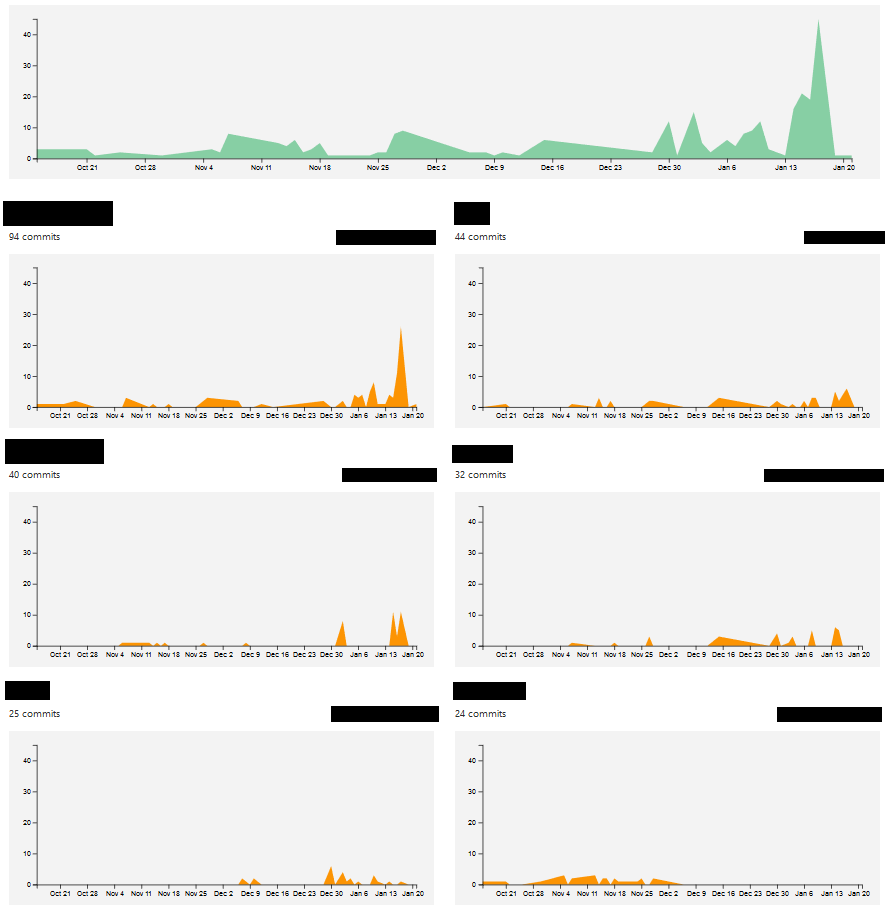
\includegraphics[scale=0.4]{slike/aktivnost.PNG} %veličina slike u odnosu na originalnu datoteku i pozicija slike
			\centering
			\caption{Primjer slike s potpisom}
			\label{fig:promjene}
		\end{figure}
		
		\begin{figure}[H]
			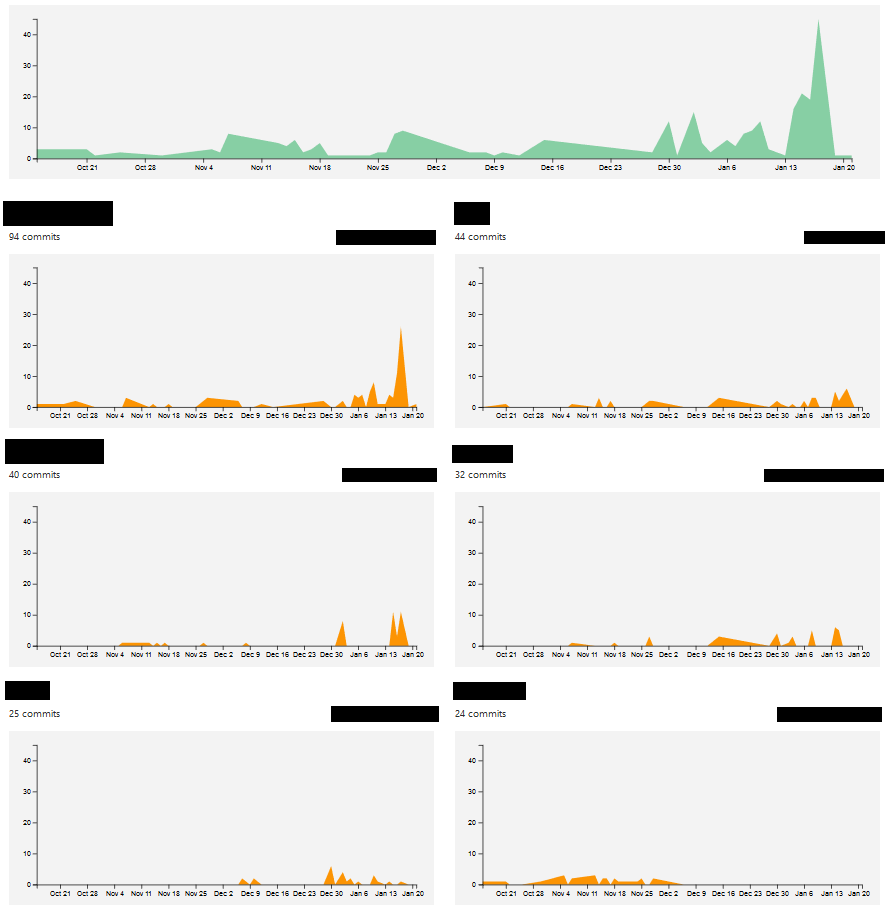
\includegraphics[width=\textwidth]{slike/aktivnost.PNG} %veličina u odnosu na širinu linije
			\caption{Primjer slike s potpisom 2}
			\label{fig:promjene2} %label mora biti drugaciji za svaku sliku
		\end{figure}
		
		Referenciranje slike \ref{fig:promjene2} u tekstu.
		
		\eject
		\fi
	
	\chapter{Specifikacija programske potpore}
		
	\section{Funkcionalni zahtjevi}
			
			\noindent \textbf{Dionici:}
			
			\begin{packed_enum}
				
				\item Neregistrirani korisnik
				\item Korisnik
				\begin{packed_enum}
					\item Vlasnik pasa
					\item Čuvar pasa
				\end{packed_enum}
				\item Administrator 				
				\item Razvojni tim
				
			\end{packed_enum}
			
			\noindent \textbf{Aktori i njihovi funkcionalni zahtjevi:}
			
			
			\begin{packed_enum}
				\item  \underbar{Neregistrirani/neprijavljeni korisnik (inicijator) može:}
				
				\begin{packed_enum}
					
					\item Na početnoj stranici pregledavati zahtjeve i oglase
					\item Odabrati željeni zahtjev/oglas i vidjeti pojedinosti tog zahtjeva/oglasa (pasmina, dob, lokacija itd.
					\item Registrirati se u sustav, stvoriti novi korisnički račun za koji mu trebaju ime, prezime, korisničko ime, e-mail adresa, lozinka, broj telefona i uloga.
				\end{packed_enum}
				
				\item  \underbar{Korisnik (inicijator) može:}
				
				\begin{packed_enum}
					
					\item Pregledavati i mijenjati osobne podatke
					\item Odjaviti se s korisničkog računa i prijaviti se nekim drugim računom
					\item Imati ulogu vlasnika pasa:
					\begin{packed_enum}
						\item Stvarati novi zahtjev za čuvanje pasa
						\item Stupiti u kontakt s potencijalnim čuvarom pasa
						\item Spremiti podatke o svom psu
						\item Ocjenjivati uslugu čuvara
						\item Pregledavati vlastite zahtjeve
					\end{packed_enum}
					\item Imati ulogu čuvara pasa:
					\begin{packed_enum}
						\item Stvarati novi oglas za čuvanje pasa
						\item Stupiti u kontakt s vlasnikom pasa
						\item Termine čuvanja pasa spremati u svoj kalendar
						\item Ocjenjivati ponašanje psa
						\item Pregledavati vlastite oglase
					\end{packed_enum}
				\end{packed_enum}
			
				\item \underbar{Administrator (inicijator) može:}
				\begin{packed_enum}
					\item Obavljati sve funkcionalnosti korisnika
					\item Dodijeliti administratorsku ulogu drugim korisnicima
					\item Odobriti ili odbaciti zahtjev/oglas
					\item Blokirati korisnika koji narušava pravila sustava
				\end{packed_enum}
			
				\item \underbar{Baza podataka (sudionik) može:}
				\begin{packed_enum}
					\item Pohraniti sve podatke o korisnicima i njihovim ulogama
					\item Pohraniti sve podatke o psima
					\item Pohraniti sve podatke o provedenim oglasima i zahtjevima
					\item Pohraniti podatke o mogućima aktivnostima sa psima
				\end{packed_enum}
			
			\end{packed_enum}
			
			\eject 
			
			
				
			\subsection{Obrasci uporabe}
				
				\subsubsection{Opis obrazaca uporabe}					

					\noindent \underbar{\textbf{UC01 - Pregledavanje zahtjeva/oglasa}}
					\begin{packed_item}
	
						\item \textbf{Glavni sudionik: } Neregistrirani korisnik 
						\item  \textbf{Cilj:} Pregledati ponuđene oglase i zahtjeve
						\item  \textbf{Sudionici:} Baza podataka 
						\item  \textbf{Preduvjet:} -
						\item  \textbf{Opis osnovnog tijeka:}
						
						\item[] \begin{packed_enum}
	
							\item Prilikom učitavanja aplikacije prikazuje se lista zahtjeva i lista oglasa
							\item Klikom na zahtjev/oglas prikazuju se dodatne informacije o tom zahtjevu/oglasu
				
						\end{packed_enum}
					\end{packed_item}
					
					\noindent \underbar{\textbf{UC02 - Registracija}}
					\begin{packed_item}
						
						\item \textbf{Glavni sudionik: } Neregistrirani korisnik 
						\item  \textbf{Cilj:} Stvoriti korisnički račun za korištenje svih funkcionalnosti aplikacije
						\item  \textbf{Sudionici:} Baza podataka 
						\item  \textbf{Preduvjet:} -
						\item  \textbf{Opis osnovnog tijeka:}
						
						\item[] \begin{packed_enum}
							
							\item Korisnik pristupa padajućem izborniku i odabire opciju za registraciju 
							\item Korisnik unosi korisničke podatke potrebne za registraciju i potvrđuje upis
							\item Korisnik dobiva povratnu informaciju o uspješnoj registraciji i preusmjerava se na početnu stranicu
							\item Korisnik se upisuje u bazu podataka
							
						\end{packed_enum}
						
						\item  \textbf{Opis mogućih odstupanja:}
						
						\item[] \begin{packed_item}
	
							\item[2.a] Odabir već zauzetog korisničkog imena i/ili e-maila, unos korisničkih podataka u neispravnom formatu, nepodudaranje lozinki 
							\item[] \begin{packed_enum}
								
								\item Sustav obavještava korisnika o neuspjelom upisu i vraća ga na stranicu za registraciju 
								\item Korisnik mijenja potrebne podatke te završava unos ili odustaje od registracije
								
							\end{packed_enum}
							
							
						\end{packed_item}
					\end{packed_item}
				
					\noindent \underbar{\textbf{UC03 - Prijava}}
					\begin{packed_item}
					
						\item \textbf{Glavni sudionik: } Korisnik 
						\item  \textbf{Cilj:} Dobivanje pristupa svim funkcionalnostima aplikacije
						\item  \textbf{Sudionici:} Baza podataka 
						\item  \textbf{Preduvjet:} Korisnik je pohranjen u bazu podataka
						\item  \textbf{Opis osnovnog tijeka:}
					
						\item[] \begin{packed_enum}
						
							\item Korisnik pristupa padajućem izborniku i odabire opciju za prijavu 
							\item Korisnik unosi korisničko ime i lozinku te potvrđuje upis
							\item Korisnik dobiva povratnu informaciju o uspješnoj prijavi i preusmjerava se na početnu stranicu
						
						\end{packed_enum}
					
						\item  \textbf{Opis mogućih odstupanja:}
					
						\item[] \begin{packed_item}
						
							\item[2.a] Neispravni unos korisničkog imena i/ili lozinke  
							\item[] \begin{packed_enum}
							
								\item Sustav obavještava korisnika o neuspjelom upisu i vraća ga na stranicu za prijavu  
								\item Korisnik unosi ispravne podatke za prijavu ili odustaje od prijave
							
							\end{packed_enum}
						\end{packed_item}
					\end{packed_item}
				
					\noindent \underbar{\textbf{UC04 - Odjava iz sustava}}
					\begin{packed_item}
						
						\item \textbf{Glavni sudionik: } Korisnik 
						\item  \textbf{Cilj:} Odjaviti se iz sustava
						\item  \textbf{Sudionici:} Baza podataka 
						\item  \textbf{Preduvjet:} Korisnik je prijavljen
						\item  \textbf{Opis osnovnog tijeka:}
						
						\item[] \begin{packed_enum}
							
							\item Korisnik pristupa padajućem izborniku i odabire opciju „Odjava“ 
							\item Aplikacija korisnika odjavljuje s trenutnog korisničkog računa
							\item Korisnik se preusmjerava na početnu stranicu gdje mu se pruža lista zahtjeva i oglasa
							
						\end{packed_enum}
					\end{packed_item}
				
					\noindent \underbar{\textbf{UC05 - Pregled osobnih podataka}}
					\begin{packed_item}
						
						\item \textbf{Glavni sudionik: } Korisnik 
						\item  \textbf{Cilj:} Pregledati osobne podatke
						\item  \textbf{Sudionici:} Baza podataka 
						\item  \textbf{Preduvjet:} Korisnik je prijavljen
						\item  \textbf{Opis osnovnog tijeka:}
						
						\item[] \begin{packed_enum}
							
							\item Korisnik pristupa padajućem izborniku i odabire opciju „Moj račun“ 
							\item Aplikacija prikazuje osobne podatke korisnika
							
						\end{packed_enum}
					\end{packed_item}
					
					\iffalse
					\noindent \underbar{\textbf{UC06 - Promjena osobnih podataka}}
					\begin{packed_item}
						
						\item \textbf{Glavni sudionik: } Korisnik 
						\item  \textbf{Cilj:} Promijeniti osobne podatke
						\item  \textbf{Sudionici:} Baza podataka 
						\item  \textbf{Preduvjet:} Korisnik je prijavljen
						\item  \textbf{Opis osnovnog tijeka:}
						
						\item[] \begin{packed_enum}
							
							\item Korisnik pristupa padajućem izborniku i odabire opciju „Moj račun“  
							\item Korisnik odabire opciju uredi osobne podatke
							\item Korisnik mijenja osobne podatke
							\item Korisnik sprema promjene
							\item Baza podataka se ažurira
							
						\end{packed_enum}
						
						\item  \textbf{Opis mogućih odstupanja:}
						
						\item[] \begin{packed_item}
							
							\item[4.a] Korisnik promijeni svoje osobne podatke, ali ne odabere opciju ”Spremi” 
							\item[] \begin{packed_enum}
								
								\item Promjene se ne spremaju
								
							\end{packed_enum}
						\end{packed_item}
					\end{packed_item}
					\fi
					
					\noindent \underbar{\textbf{UC06 – Dodavanje pasa}}
					\begin{packed_item}
						
						\item \textbf{Glavni sudionik: } Korisnik (vlasnik pasa)
						\item  \textbf{Cilj:} Dodavanje pasa na web stranicu
						\item  \textbf{Sudionici:} Baza podataka 
						\item  \textbf{Preduvjet:} Korisnik je prijavljen, korisnik ima ulogu vlasnika pasa
						\item  \textbf{Opis osnovnog tijeka:}
						
						\item[] \begin{packed_enum}
							
							\item Korisnik na padajućem izborniku odabire opciju "Moji psi" 
							\item Korisnik na stranici s prikazom vlastitih pasa pritiskuje gumb "Dodaj pasa"
							\item Korisnik ispunjava osobne podatke o pasu
							\item Korisnik pritiskuje gumb "Spremi"
							\item Podaci o pasu se spremaju u sustav
							
						\end{packed_enum}
					
				
						\item  \textbf{Opis mogućih odstupanja:}
		
						\item[] \begin{packed_item}
	
							\item[4.a] Korisnik zaboravlja pritisnuti gumb "Spremi"
							\item[] \begin{packed_enum}
								\item Podaci o pasu se ne spremaju u sustav
							\end{packed_enum}
						\end{packed_item}
					\end{packed_item}
					
					\noindent \underbar{\textbf{UC07 – Pregledavanje tuđih zahtjeva}}
					\begin{packed_item}
						
						\item \textbf{Glavni sudionik: } Korisnik 
						\item  \textbf{Cilj:} Pronalaženje najprikladnijeg zahtjeva
						\item  \textbf{Sudionici:} Baza podataka 
						\item  \textbf{Preduvjet:} Korisnik je prijavljen, korisnik ima ulogu čuvara
						\item  \textbf{Opis osnovnog tijeka:}
						
						\item[] \begin{packed_enum}
							
							\item Korisnik na početnoj stranici prolazi kroz listu tuđih zahtjeva 
							\item Korisnik odabire odgovarajući zahtjev
							\item Korisnik pregledava dodatne podatke o tom zahtjevu
							
						\end{packed_enum}
					\end{packed_item}
				
					\noindent \underbar{\textbf{UC08 – Pregledavanje tuđih oglasa}}
					\begin{packed_item}
						
						\item \textbf{Glavni sudionik: } Korisnik 
						\item  \textbf{Cilj:} Pronalaženje najprikladnijeg oglasa
						\item  \textbf{Sudionici:} Baza podataka 
						\item  \textbf{Preduvjet:} Korisnik je prijavljen, korisnik ima ulogu vlasnika
						\item  \textbf{Opis osnovnog tijeka:}
						
						\item[] \begin{packed_enum}
							
							\item Korisnik na početnoj stranici prolazi kroz listu tuđih oglasa  
							\item Korisnik odabire odgovarajući oglas
							\item Korisnik pregledava dodatne podatke o tom oglasu
							
						\end{packed_enum}
					\end{packed_item}

					\noindent \underbar{\textbf{UC09 – Pregledavanje vlastitih zahtjeva}}
					\begin{packed_item}
						
						\item \textbf{Glavni sudionik: } Korisnik (vlasnik pasa)
						\item  \textbf{Cilj:} Pregledavanje svojih kreiranih zahtjeva
						\item  \textbf{Sudionici:} Baza podataka 
						\item  \textbf{Preduvjet:} Korisnik je prijavljen, korisnik ima ulogu vlasnika
						\item  \textbf{Opis osnovnog tijeka:}
						
						\item[] \begin{packed_enum}
							
							\item Korisnik pristupa padajućem izborniku i odabire opciju „Moji zahtjevi“  
							\item Korisniku se prikazuje lista zahtjeva
							
						\end{packed_enum}
					
						\item  \textbf{Opis mogućih odstupanja:}
						
						\item[] \begin{packed_item}
							
							\item[2.a] Korisnik nema kreiranih zahtjeva
							\item[] \begin{packed_enum}
								
								\item Korisniku se prikazuje prikladna poruka
								
							\end{packed_enum}
						\end{packed_item}
					\end{packed_item}	
				
					\noindent \underbar{\textbf{UC10 – Pregledavanje vlastitih oglasa}}
					\begin{packed_item}
						
						\item \textbf{Glavni sudionik: } Korisnik (čuvar pasa)
						\item  \textbf{Cilj:} Pregledavanje svojih kreiranih oglasa
						\item  \textbf{Sudionici:} Baza podataka 
						\item  \textbf{Preduvjet:} Korisnik je prijavljen, korisnik ima ulogu čuvara
						\item  \textbf{Opis osnovnog tijeka:}
						
						\item[] \begin{packed_enum}
							
							\item Korisnik pristupa padajućem izborniku i odabire opciju „Moji oglasi“  
							\item Korisniku se prikazuje lista oglasa
							
						\end{packed_enum}
						
						\item  \textbf{Opis mogućih odstupanja:}
						
						\item[] \begin{packed_item}
							
							\item[2.a] Korisnik nema kreiranih oglasa
							\item[] \begin{packed_enum}
								
								\item Korisniku se prikazuje prikladna poruka
								
							\end{packed_enum}
						\end{packed_item}
					\end{packed_item}	
				
					\noindent \underbar{\textbf{UC11 – Kreiranje novog zahtjeva}}
					\begin{packed_item}
						
						\item \textbf{Glavni sudionik: } Korisnik (vlasnik pasa)
						\item  \textbf{Cilj:} Objavljivanje novog zahtjeva za čuvanje pasa
						\item  \textbf{Sudionici:} Baza podataka, administrator
						\item  \textbf{Preduvjet:} Korisnik je prijavljen, korisnik ima ulogu vlasnika
						\item  \textbf{Opis osnovnog tijeka:}
						
						\item[] \begin{packed_enum}
							
							\item Korisnik na početnoj stranici odabire opciju za kreiranje novog zahtjeva   
							\item Korisniku se otvara stranica za kreiranje zahtjeva
							\item Korisnik unosi sve tražene podatke za kreiranje zahtjeva (pasmina, dob, period čuvanja itd.)
							\item Korisnik odabire opciju za objavljivanje zahtjeva
							\item Zahtjev se šalje administratoru na uvid
							
						\end{packed_enum}
						
						\item  \textbf{Opis mogućih odstupanja:}
						
						\item[] \begin{packed_item}
							
							\item[4.a] Korisnik nije ispravno unio sve podatke
							\item[] \begin{packed_enum}
								
								\item Korisnika se ponovno vraća na stranicu za kreiranje zahtjeva s odgovarajućom porukom o greški 
								
							\end{packed_enum}
						\end{packed_item}
					\end{packed_item}		
				
					\noindent \underbar{\textbf{UC12 – Kreiranje novog oglasa}}
					\begin{packed_item}
						
						\item \textbf{Glavni sudionik: } Korisnik (čuvar pasa)
						\item  \textbf{Cilj:} Objavljivanje novog oglasa  za čuvanje pasa
						\item  \textbf{Sudionici:} Baza podataka, administrator
						\item  \textbf{Preduvjet:} Korisnik je prijavljen, korisnik ima ulogu čuvara
						\item  \textbf{Opis osnovnog tijeka:}
						
						\item[] \begin{packed_enum}
							
							\item Korisnik na početnoj stranici odabire opciju za kreiranje novog oglasa     
							\item Korisniku se otvara stranica za kreiranje oglasa  
							\item Korisnik unosi sve tražene podatke za kreiranje oglasa   (preferirana pasmina, preferirana dob, period čuvanja itd.)
							\item Korisnik odabire opciju za objavljivanje oglasa
							\item Oglas se šalje administratoru na uvid
							
						\end{packed_enum}
						
						\item  \textbf{Opis mogućih odstupanja:}
						
						\item[] \begin{packed_item}
							
							\item[4.a] Korisnik nije ispravno unio sve podatke
							\item[] \begin{packed_enum}
								
								\item Korisnika se ponovno vraća na stranicu za kreiranje oglasa s odgovarajućom porukom o greški 
								
							\end{packed_enum}
						\end{packed_item}
					\end{packed_item}	
				
					\noindent \underbar{\textbf{UC13 – Pronalaženje najboljeg odabira čuvara pasa}}
					\begin{packed_item}
						
						\item \textbf{Glavni sudionik: } Korisnik (vlasnik pasa)
						\item  \textbf{Cilj:} Pronalaženje najprikladnijeg čuvara pasa
						\item  \textbf{Sudionici:} Baza podataka, korisnik (čuvar pasa)
						\item  \textbf{Preduvjet:} Korisnikov zahtjev je potvrđen od administratora
						\item  \textbf{Opis osnovnog tijeka:}
						
						\item[] \begin{packed_enum}
							
							\item Korisnik pristupa padajućem izborniku i odabire opciju „Moji zahtjevi“    
							\item Korisnik na listi zahtjeva pokraj željenog zahtjeva pritišće gumb "Pronalaženje najboljeg odabira"  
							\item Korisnik (čuvar) dobiva obavijest sa najpogodnijim zahtjevom
							\item Korisnici prihvaćaju odabir
							\item Korisnici razmjenjuju detalje
							
						\end{packed_enum}
					
						\item  \textbf{Opis mogućih odstupanja:}
			
							\item[] \begin{packed_item}
							\item[4.a] Korisnik (vlasnik) odbija zahtjev
							\item[] \begin{packed_enum}
			
								\item Daljnja suradnja između korisnika nije moguća
			
							\end{packed_enum}
						
							\item[4.b] Korisnik (čuvar) odbija zahtjev
							\item[] \begin{packed_enum}
								
								\item Daljnja suradnja između korisnika nije moguća
								
							\end{packed_enum}
						\end{packed_item}
					\end{packed_item}	
				
					\noindent \underbar{\textbf{UC14 – Pronalaženje najboljeg odabira vlasnika pasa}}
					\begin{packed_item}
						
						\item \textbf{Glavni sudionik: } Korisnik (čuvar pasa)
						\item  \textbf{Cilj:} Pronalaženje najprikladnijeg pasa za čuvanje
						\item  \textbf{Sudionici:} Baza podataka, korisnik (vlasnik pasa)
						\item  \textbf{Preduvjet:} Korisnikov oglas je potvrđen od administratora
						\item  \textbf{Opis osnovnog tijeka:}
						
						\item[] \begin{packed_enum}
							
							\item Korisnik pristupa padajućem izborniku i odabire opciju „Moji oglasi“    
							\item Korisnik na listi oglasa pokraj željenog oglasa pritišće gumb "Pronalaženje najboljeg odabira"  
							\item Korisnik (vlasnik) dobiva obavijest sa najboljim odabirom
							\item Korisnici prihvaćaju odabir
							\item Korisnici razmjenjuju detalje
							
						\end{packed_enum}
						
						\item  \textbf{Opis mogućih odstupanja:}
						
						\item[] \begin{packed_item}
							
							\item[4.a] Korisnik (vlasnik) odbija zahtjev
							\item[] \begin{packed_enum}
								
								\item Daljnja suradnja između korisnika nije moguća
								
							\end{packed_enum}
							\item[4.b] Korisnik (čuvar) odbija zahtjev
							\item[] \begin{packed_enum}
								
								\item Daljnja suradnja između korisnika nije moguća
								
							\end{packed_enum}
						\end{packed_item}
					\end{packed_item}	
				
					\noindent \underbar{\textbf{UC15 – Javljanje na oglas}}
					\begin{packed_item}
						
						\item \textbf{Glavni sudionik: } Korisnik (vlasnik pasa)
						\item  \textbf{Cilj:} Pronalaženje najprikladnijeg čuvara pasa
						\item  \textbf{Sudionici:} Baza podataka, korisnik (čuvar pasa)
						\item  \textbf{Preduvjet:} Korisnikov zahtjev je potvrđen od administratora
						\item  \textbf{Opis osnovnog tijeka:}
						
						\item[] \begin{packed_enum}
							
							\item Korisnik na početnoj stranici prolazi kroz listu tuđih oglasa   
							\item Korisnik odabire odgovarajući oglas
							\item Korisnik pregledava dodatne podatke o tom oglasu
							\item Korisnik odabire oglas 
							\item Korisniku (čuvaru) se šalje obavijest o odabiru
							\item Korisnik (čuvar) prihvaća odabir
							\item Korisnici razmjenjuju detalje
							
						\end{packed_enum}
						
						\item  \textbf{Opis mogućih odstupanja:}
						
						\item[] \begin{packed_item}
							
							\item[4.a] Korisniku se ne sviđa oglas (ne odabire oglas)
							\item[] \begin{packed_enum}
								
								\item Korisnik se vraća na početnu listu
								\item Korisnik nastavlja pretraživat
								
							\end{packed_enum}
						
							\item[6.a] Korisnik (čuvar) odbija zahtjev 
							\item[] \begin{packed_enum}
								
								\item Daljnja suradnja između korisnika nije moguća
								
							\end{packed_enum}
						\end{packed_item}
					\end{packed_item}	

					\noindent \underbar{\textbf{UC16 – Javljanje na zahtjev}}
					\begin{packed_item}
						
						\item \textbf{Glavni sudionik: } Korisnik (čuvar pasa)
						\item  \textbf{Cilj:} Pronalaženje najprikladnijeg pasa za čuvanje
						\item  \textbf{Sudionici:} Baza podataka, korisnik (vlasnik pasa)
						\item  \textbf{Preduvjet:} Korisnikov oglas je potvrđen od administratora
						\item  \textbf{Opis osnovnog tijeka:}
						
						\item[] \begin{packed_enum}
							
							\item Korisnik na početnoj stranici prolazi kroz listu tuđih zahtjeva   
							\item Korisnik odabire odgovarajući zahtjev
							\item Korisnik pregledava dodatne podatke o tom zahtjevu
							\item Korisnik odabire zahtjev 
							\item Korisniku(vlasniku) se šalje obavijest o odabiru
							\item Korisnik (vlasnik) prihvaća odabir
							\item Korisnici razmjenjuju detalje
							
						\end{packed_enum}
						
						\item  \textbf{Opis mogućih odstupanja:}
						
						\item[] \begin{packed_item}
							
							\item[4.a] Korisniku se ne sviđa zahtjev (ne odabire zahtjev)
							\item[] \begin{packed_enum}
								
								\item Korisnik se vraća na početnu listu
								\item Korisnik nastavlja pretraživat
								
							\end{packed_enum}
							
							\item[6.a] Korisnik (vlasnik) odbija zahtjev 
							\item[] \begin{packed_enum}
								
								\item Daljnja suradnja između korisnika nije moguća
								
							\end{packed_enum}
						\end{packed_item}
					\end{packed_item}	
					
					\noindent \underbar{\textbf{UC17 - Unos dogovorenih termina u kalendar}}	
					\begin{packed_item}
						
						\item \textbf{Glavni sudionik: } Korisnik (čuvar pasa)
						\item  \textbf{Cilj:} Popunjavanje kalendara radi bolje organizacije vremena
						\item  \textbf{Sudionici:} Baza podataka
						\item  \textbf{Preduvjet:} Korisnik(vlasnik pasa) i korisnik(čuvar pasa) su dogovorili termin 
						\item  \textbf{Opis osnovnog tijeka:}
						
						\item[] \begin{packed_enum}
							
							\item Korisnik u padajućem izborniku odabire opciju 'Moj račun'   
							\item Korisnik pohranjuje dogovoreni termin u kalendar
							\item Korisnik sprema kalendar
							
						\end{packed_enum}
						
						\item  \textbf{Opis mogućih odstupanja:}
						
						\item[] \begin{packed_item}
							
							\item[3.a] Korisniku ne sprema kalendar
							\item[] \begin{packed_enum}
								
								\item Promjene se ne spremaju
								
							\end{packed_enum}
							
						\end{packed_item}
					\end{packed_item}	
					
					\noindent \underbar{\textbf{UC18 - Ocjenjivanje usluge čuvanja}}
					\begin{packed_item}
						
						\item \textbf{Glavni sudionik: } Korisnik (vlasnik pasa)
						\item  \textbf{Cilj:} Pružiti informaciju vlasnicima pasa kakav je čuvar
						\item  \textbf{Sudionici:} Baza podataka
						\item  \textbf{Preduvjet:} Korisnik(vlasnik pasa) i korisnik(čuvar pasa) imali su poslovni odnos 
						\item  \textbf{Opis osnovnog tijeka:}
						
						\item[] \begin{packed_enum}
							
							\item Korisnik u padajućem izborniku odabire opciju "Prošla čuvanja"
							\item Korisnik odabire željeno čuvanje
							\item Korisnik ocjenjuje iskustvo s čuvarom pasa
							
						\end{packed_enum}
					\end{packed_item}	
					
					\noindent \underbar{\textbf{UC19 - Ocjenjivanje ponašanja psa}}
					\begin{packed_item}
						
						\item \textbf{Glavni sudionik: } Korisnik (čuvar pasa)
						\item  \textbf{Cilj:} Pružiti informaciju čuvarima pasa kakav je pas
						\item  \textbf{Sudionici:} Baza podataka
						\item  \textbf{Preduvjet:} Korisnik(vlasnik pasa) i korisnik(čuvar pasa) imali su poslovni odnos 
						\item  \textbf{Opis osnovnog tijeka:}
						
						\item[] \begin{packed_enum}
							
							\item Korisnik u padajućem izborniku odabire opciju "Prošla čuvanja"
							\item Korisnik odabire željeno čuvanje
							\item Korisnik ocjenjuje iskustvo s vlasnikom pasa
							
						\end{packed_enum}
					\end{packed_item}	
					
					\noindent \underbar{\textbf{UC20 - Dodjeljivanje administratorske uloge korisniku}}
					\begin{packed_item}
						
						\item \textbf{Glavni sudionik: } Administrator
						\item  \textbf{Cilj:} Pružiti korisniku administratorsku ulogu
						\item  \textbf{Sudionici:} Baza podataka
						\item  \textbf{Preduvjet:} -
						\item  \textbf{Opis osnovnog tijeka:}
						
						\item[] \begin{packed_enum}
							
							\item Administrator preko padajućeg izbornika pristupa stranici za administratorsko upravljanje
							\item Administrator u listi korisnika pronalazi željenog korisnika
							\item Administrator odabranom korisniku dodjeljuje administratorsku ulogu
							
						\end{packed_enum}
					\end{packed_item}	
					
					\noindent \underbar{\textbf{UC21 - Potvrđivanje stvorenog zahtjeva}}
					\begin{packed_item}
						
						\item \textbf{Glavni sudionik: } Administrator
						\item  \textbf{Cilj:} Potvrditi stvoreni zahtjev da se može objaviti
						\item  \textbf{Sudionici:} Baza podataka
						\item  \textbf{Preduvjet:} Korisnik(vlasnik pasa) je stvorio zahtjev
						\item  \textbf{Opis osnovnog tijeka:}
						
						\item[] \begin{packed_enum}
							
							\item Administrator preko padajućeg izbornika pristupa stranici za administratorsko upravljanje
							\item Administrator u listi 'Zahtjevi u tijeku' pronalazi željeni zahtjev
							\item Administrator pritiskom na gumb 'Potvrdi' potvrđuje zahtjev
							\item Zahtjev se objavljuje
							
						\end{packed_enum}
						\item  \textbf{Opis mogućih odstupanja:}
						
						\item[] \begin{packed_item}
							
							\item[3.a] Administrator smatra zahtjev nevaljanim
							\item[] \begin{packed_enum}
								
								\item Administrator pritiskom na gumb 'Odbij' odbija zahtjev
								\item Zahtjev se briše 
								
							\end{packed_enum}
							
						\end{packed_item}
					\end{packed_item}
					
					\noindent \underbar{\textbf{UC22 - Potvrđivanje stvorenog oglasa}}
					\begin{packed_item}
						
						\item \textbf{Glavni sudionik: } Administrator
						\item  \textbf{Cilj:} Potvrditi stvoreni oglas da se može objaviti
						\item  \textbf{Sudionici:} Baza podataka
						\item  \textbf{Preduvjet:} Korisnik(čuvar pasa) je stvorio oglas
						\item  \textbf{Opis osnovnog tijeka:}
						
						\item[] \begin{packed_enum}
							
							\item Administrator preko padajućeg izbornika pristupa stranici za administratorsko upravljanje
							\item Administrator u listi 'Oglasi u tijeku' pronalazi željeni oglas
							\item Administrator pritiskom na gumb 'Potvrdi' potvrđuje oglas
							\item Oglas se objavljuje
							
						\end{packed_enum}
						\item  \textbf{Opis mogućih odstupanja:}
						
						\item[] \begin{packed_item}
							
							\item[3.a] Administrator smatra oglas nevaljanim
							\item[] \begin{packed_enum}
								
								\item Administrator pritiskom na gumb 'Odbij' odbija oglas
								\item Oglas se briše 
								
							\end{packed_enum}
							
						\end{packed_item}
					\end{packed_item}
					
					\noindent \underbar{\textbf{UC23 - Blokiranje korisnika}}
					\begin{packed_item}
						
						\item \textbf{Glavni sudionik: } Administrator
						\item  \textbf{Cilj:} Blokirati korisnika radi narušavanja pravila sustava
						\item  \textbf{Sudionici:} Baza podataka
						\item  \textbf{Preduvjet:} Korisnik je narušio pravila sustava
						\item  \textbf{Opis osnovnog tijeka:}
						
						\item[] \begin{packed_enum}
							
							\item Administrator preko padajućeg izbornika pristupa stranici za administratorsko upravljanje
							\item Administrator u listi korisnika pronalazi željenog korisnika
							\item Administrator blokira odabranog korisnika
							
						\end{packed_enum}
					\end{packed_item}	
				\eject				
				\subsubsection{Dijagrami obrazaca uporabe}
					
					\begin{figure}[htb]
						\centering
						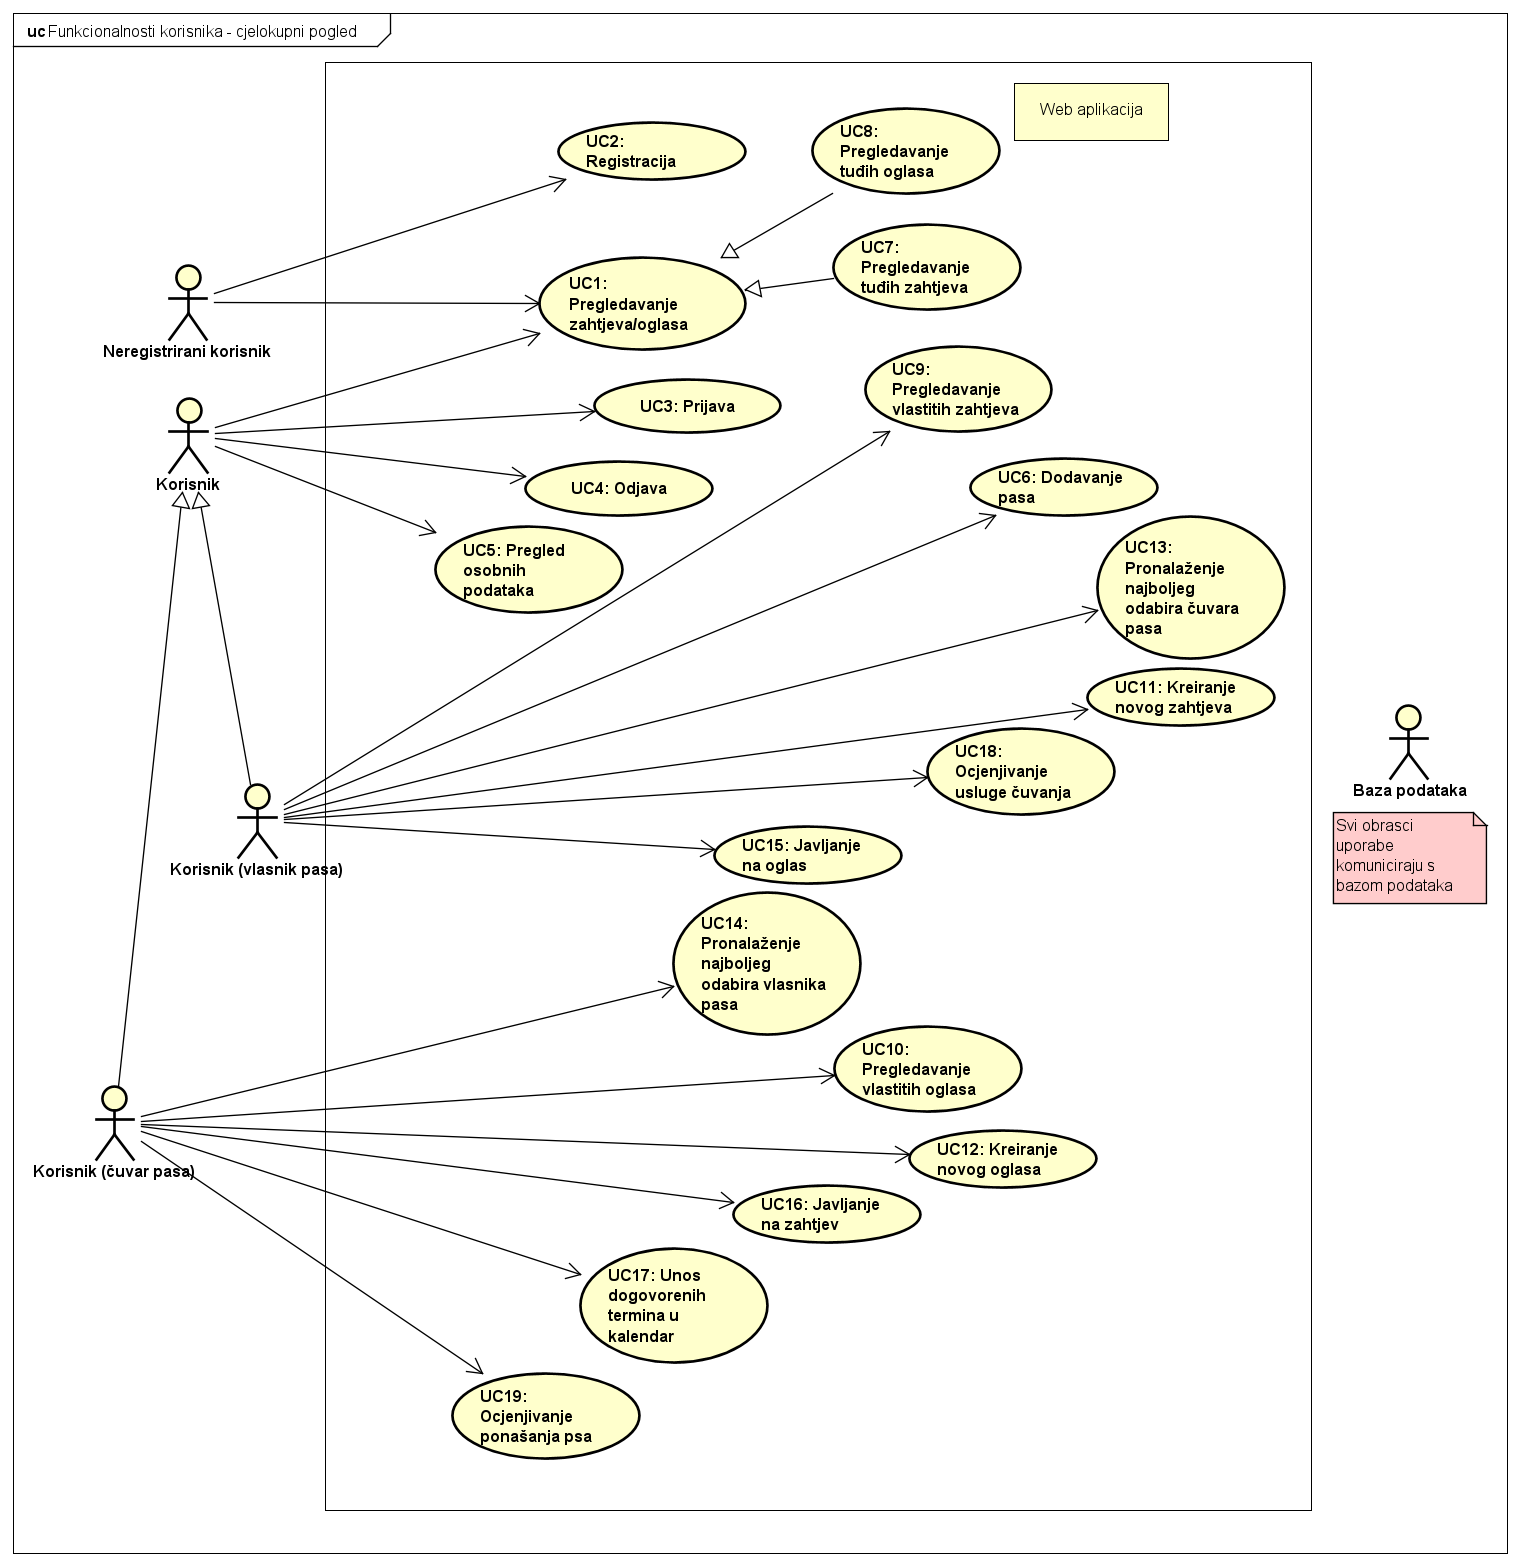
\includegraphics[width=12cm]{slike/korisnikExport}
						\caption{Dijagram obrasca uporabe, funkcionalnost neregistriranog korisnika i korisnika (vlasnika pasa i čuvara pasa)}
						\label{fig:DOU-korisnici}
					\end{figure}
				\eject		
					\begin{figure}[htb]
						\centering
						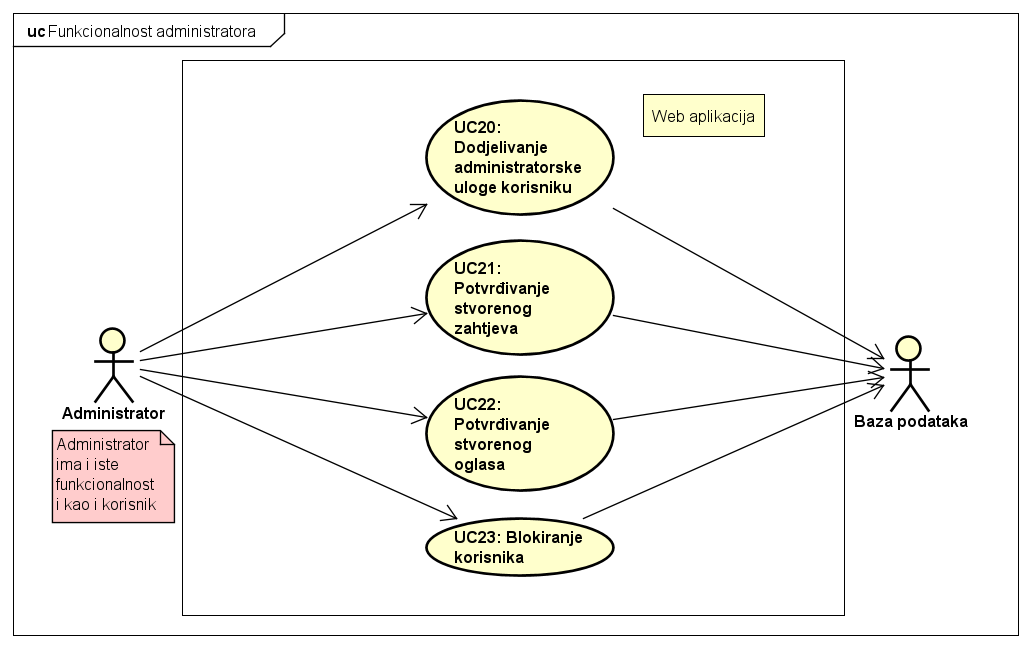
\includegraphics[width=12cm]{slike/dijagramExport}
						\caption{Dijagram obrasca uporabe, funkcionalnost administratora}
						\label{fig:DOU-administrator}
					\end{figure}
				\eject		
				
			\subsection{Sekvencijski dijagrami}
				
				\textbf{Obrazac uporabe UC11 - Kreiranje novog zahtjeva}\\
				
				Korisnik (vlasnik pasa) na početnoj stranici odabire opciju za kreiranje novog zahtjeva. Web aplikacija mu otvara stranicu za kreiranje zahtjeva. Korisnik tamo unosi tražene podatke (pasmina, dob, period čuvanja, itd.) za kreiranje zahtjeva. Potom korisnik potvrđuje kreiranje zahtjeva. Ako korisnik nije ispravno unio podatke, prilikom potvrde web aplikacija ga ponovno usmjerava na istu stranicu s prikladnom porukom o greški. Web aplikacija mu daje odgovor o uspješnom kreiranju zahtjeva. Zahtjev se pohranjuje u bazu podataka.
				
				\begin{figure}[htb]
					\centering
					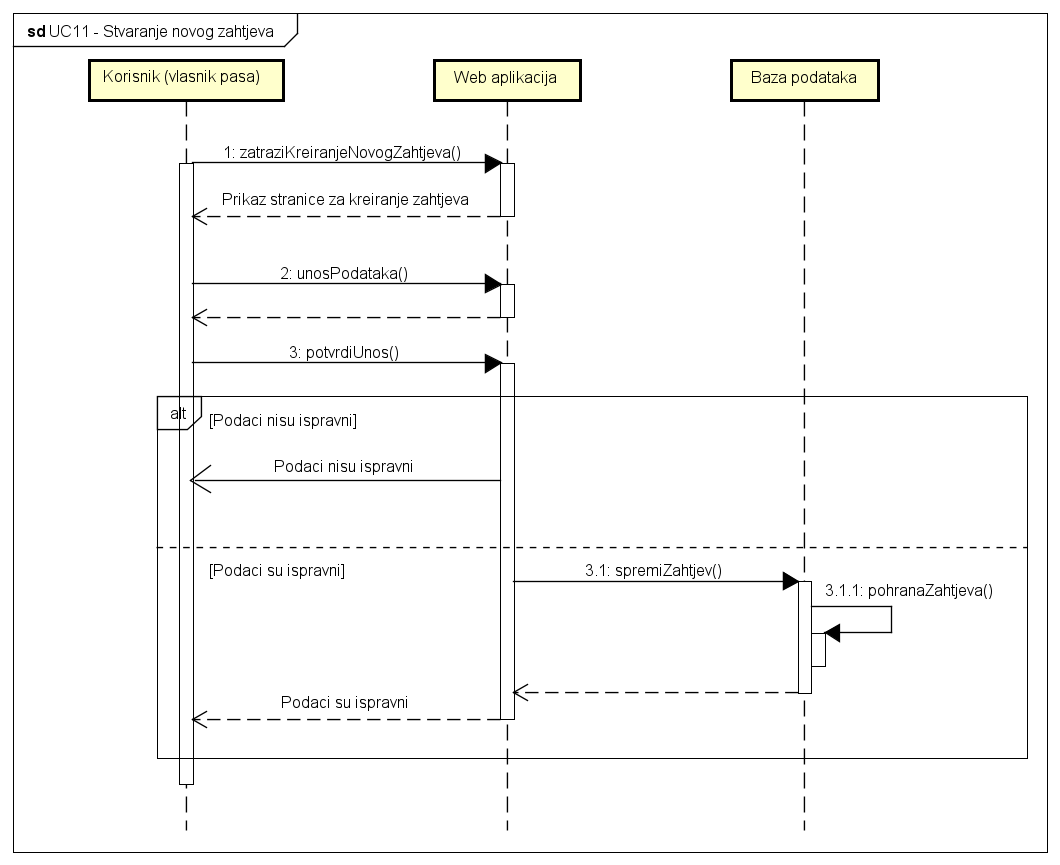
\includegraphics[width=16cm]{slike/UC11 - Stvaranje novog zahtjeva - sekvencijski - v3}
					\caption{Sekvencijski dijagram za UC11}
					\label{fig:Sekvencijski-UC11}
				\end{figure}
				\eject		
				
				\textbf{Obrazac uporabe UC14 - Pronalaženje najboljeg odabira vlasnika pasa}\\
				
				Korisnik (čuvar pasa) na početnoj stranici odabire opciju "Moji oglasi". Web aplikacija mu otvara stranicu s njegovim oglasima. Korisnik tamo pokraj željenog oglasa pritišće gumb "Pronalaženje najboljeg odabira". Web aplikacija pronalazi najboljeg vlasnika pasa i šalje ga korisniku. Korisnik ima mogućnost ga prihvatiti, ali i odbiti. Ako korisnik odbije, nema daljnje suradnje s vlasnikom pasa. Ako ga korisnik prihvati, obavijest se šalje vlasniku pasa da je došlo do najboljeg odabira. Tamo vlasnik pasa ima također opciju prihvatiti suradnju kao i odbiti ju.
				
				\begin{figure}[htb]
					\centering
					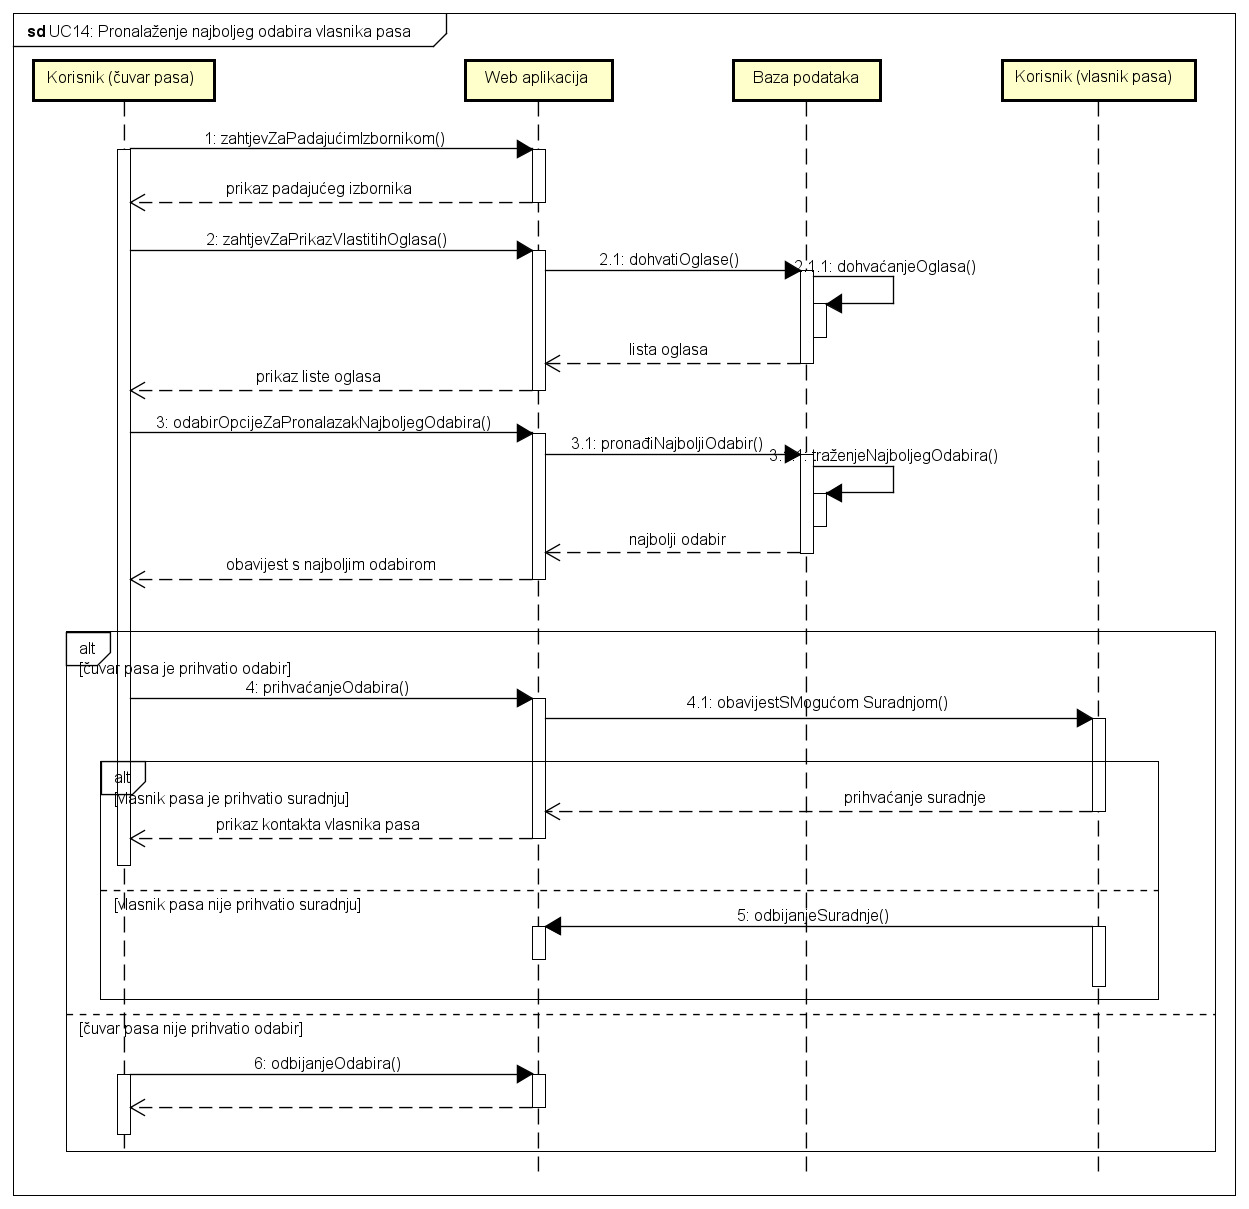
\includegraphics[width=16cm]{slike/UC14 - sekvencijski}
					\caption{Sekvencijski dijagram za UC14}
					\label{fig:Sekvencijski-UC14}
				\end{figure}
				\eject		
				
				\textbf{Obrazac uporabe UC21 - Potvrđivanje stvorenog zahtjeva}\\
				
				Administrator sustava na početnoj stranici odabire opciju za pristupanje stranici za administratorsko upravljanje. Web aplikacija šalje upit za potrebnim elementima (svi nepotvrđeni zahtjevi i oglasi te svi korisnici sustava) bazi podataka. Primitkom istih, web aplikacija otvara stranicu administratoru. Administrator u listi zahtjeva pronalazi željeni zahtjev te kraj njega pritišće gumb za njegove potvrđivanje. Web aplikacija šalje upit za ažuriranjem zahtjeva bazi podataka. Baza podataka ga ažurira i šalje ažuriranu listu zahtjeva web aplikaciji. Web aplikacija otvara ponvono stranicu administratoru, ali sada s ažuriranom listom zahtjeva.
				
				\begin{figure}[htb]
					\centering
					\includegraphics[width=16cm]{slike/UC21 - Potvrđivanje stvorenog zahtjeva - sekvencijski}
					\caption{Sekvencijski dijagram za UC21}
					\label{fig:Sekvencijski-UC21}
				\end{figure}
				\eject	
				
				\textbf{Obrazac uporabe UC23 - Blokiranje korisnika}\\
				Administrator sustava na početnoj stranici odabire opciju za pristupanje stranici za administratorsko upravljanje. Web aplikacija šalje upit za potrebnim elementima (svi nepotvrđeni zahtjevi i oglasi te svi korisnici sustava) bazi podataka. Primitkom istih, web aplikacija otvara stranicu administratoru. Administrator u listi korisnika pronalazi željenog korisnika te kraj njega pritišće gumb na njegovo blokiranje. Web aplikacija šalje upit za brisanjem korisnika u bazi podataka. Baza podataka briše korisnika i šalje ažurirana listu korisnika web aplikaciji. Web aplikacija otvara ponovno stranicu administratoru, ali sada s ažuriranom listom korisnika.
				
				\begin{figure}[htb]
					\centering
					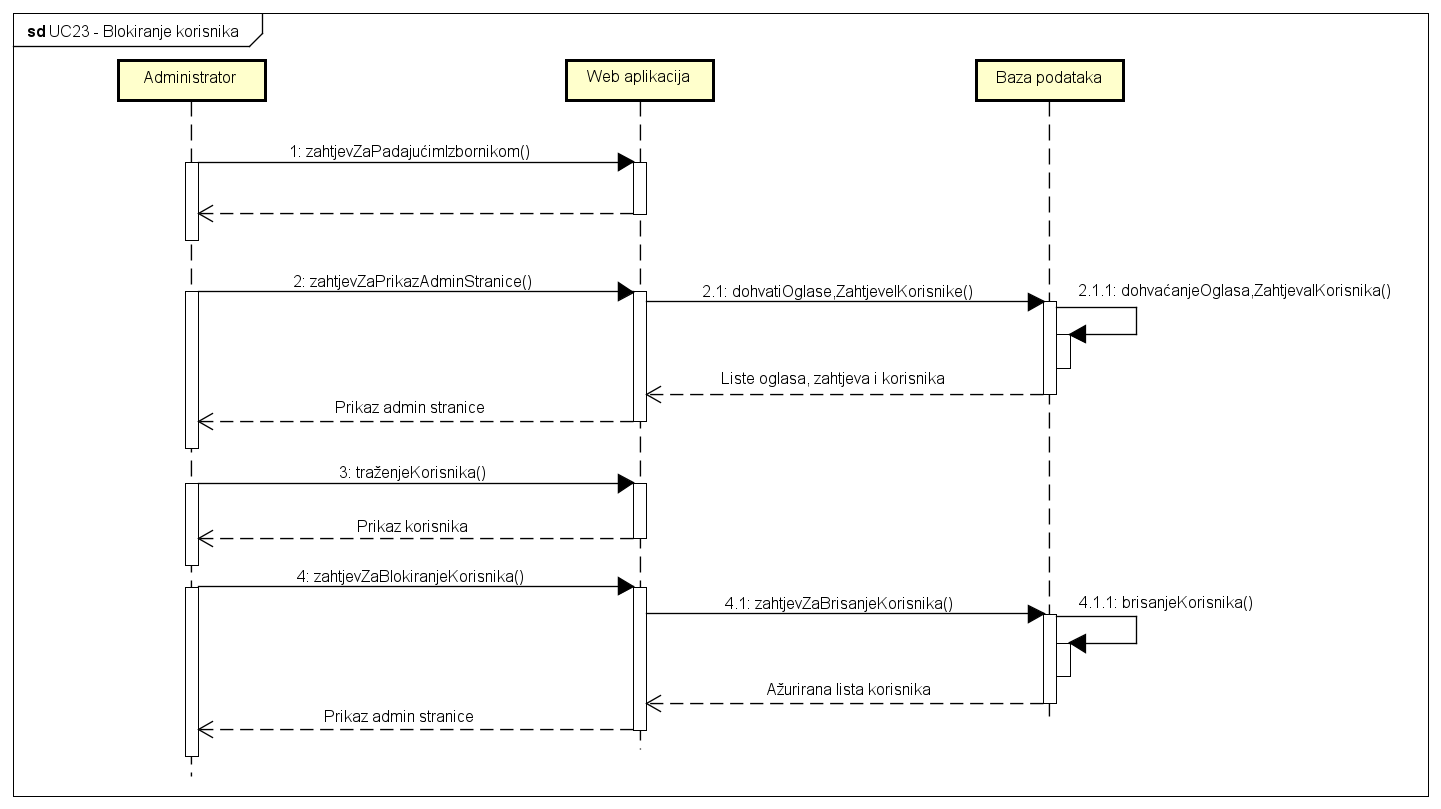
\includegraphics[width=16cm]{slike/UC23 - Blokiranje korisnika - sekvencijski}
					\caption{Sekvencijski dijagram za UC23}
					\label{fig:Sekvencijski-UC23}
				\end{figure}
				\eject	
	
		\section{Ostali zahtjevi}
		
			\textbf{\textit{dio 1. revizije}}\\
		 
			 \textit{Nefunkcionalni zahtjevi i zahtjevi domene primjene dopunjuju funkcionalne zahtjeve. Oni opisuju \textbf{kako se sustav treba ponašati} i koja \textbf{ograničenja} treba poštivati (performanse, korisničko iskustvo, pouzdanost, standardi kvalitete, sigurnost...). Primjeri takvih zahtjeva u Vašem projektu mogu biti: podržani jezici korisničkog sučelja, vrijeme odziva, najveći mogući podržani broj korisnika, podržane web/mobilne platforme, razina zaštite (protokoli komunikacije, kriptiranje...)... Svaki takav zahtjev potrebno je navesti u jednoj ili dvije rečenice.}
			 
			 
			 
	
	\chapter{Arhitektura i dizajn sustava}

		Web aplikacija "Čuvari pasa" izvedena je u arhitekturi klijent-poslužitelj. Klijenti (korisnici) šalju zahtjeve za nekom uslugom poslužitelju (web aplikaciji). Poslužitelj odgovara sa traženom uslugom ili statusom pogreške (HTTP status 404). Glavni cilj ove arhitekture je centralizirani sustav koji dijeli informacije i usluge.
		Nadalje se arhitektura može podijeliti na web poslužitelj, web preglednik i bazu podataka.\\
		\newline
		\textbf{Web poslužitelj} je zapravo funkcionalnost web aplikacije. On komunicira s klijentom preko web preglednika. Primarna uloga mu je "nabavljanje" HTTP zahtjeva i slanje HTTP odgovora. Ovisno o zahtjevu, web poslužitelj komunicira i s bazom podataka u kojoj se nalaze potrebni podaci. 
		\newline
		\textbf{Web preglednik} je softver koji služi kao sučelje između poslužitelja i klijenta i web dokumente klijentu. Njegova primarna uloga je slanje HTTP zahtjeva i primanje HTTP odgovora. Web preglednici prevode kod koji dobivaju u HTTP odgovoru te ga zatim prikazuju.
		\newline
		\textbf{Baza podataka} koristi se za sigurno spremanje podataka. Povezana je s web aplikacijom koja joj šalje upite za potrebnim podacima. Baza podataka je dalje opisana u poglavlju 4.1 Baza podataka.
		\newline
		\newline
		Web aplikacija koristi arhitekturu MVC (Model-View-Controller). \textbf{Model} predstavlja dinamičke strukture podataka. U njemu se izravno upravlja podacima.
		\textbf{View} predstavlja prikaz podataka, a \textbf{Controller} prima zahtjeve i prosljeđuje ih gdje su dalje potrebni. MVC je implementiran u našu web aplikaciju tako da su Model i Controller komponente sadržane u back-end dijelu, a view u front-end dijelu. \textbf{Front-end} (prezentacijski sloj) je dio aplikacije zaslužan za grafičko korisničko sučelje dok se \textbf{back-end} (sloj pristupa podacima) može poistovjetiti sa web poslužiteljem. U njemu se opisuju funkcionalnosti web aplikacije odnosno on upravlja web aplikacijom.\\
		Backend je osim na model (repository) i controller komponente podijeljen i na service komponentu. U njoj se nalazi implementacija poslovne logike.
		\newline
		Front-end smo odlučili raditi u programskom jeziku JavaScriptu u radnom okviru React, a back-end u programskom jeziku Javi u radnom okviru Spring Boot. Razvojna okruženja u kojima radimo su Visual Studio Code i IntelliJ.
		
		
		

	
		

		
		\eject
				
		\section{Baza podataka}
			
			Sustav koristi relacijsku bazu podataka koja će biti implementirana u PostgreSQLu. Relacijsku bazu podataka koristimo radi lakšeg oblikovanja sustava kao stvarnog svijeta, a PostgresSQl jer smo najbolje upoznati sa njime. U njoj se entiteti modeliraju kao tablice koje imaju vlastito ime i skup atributa.\\
			Baza podataka nam je potrebna zbog njezine sigurnosti podataka, ali i brzog dohvata, pohrane i izmijene podataka koje sustav koristi za daljnje akcije.
			Baza podataka ovog sustava korisit sjedeće entitete:
			\begin{packed_item}
				\item Role
				\item App User
				\item Breed
				\item Owner
				\item Guardian
				\item Dog
				\item Request Dog
				\item Request Guardian
				\item Request Guardians Dog
				\item Activity
				\item Request Activity
				\item Agreed request
				
			\end{packed_item}
			
		
			\subsection{Opis tablica}
			
			
			\textbf{Role} je entitet koji sadržava sve važne informacije o rolama aplikacije. Povezan je vezom One-To-Many s tablicom App User preko atributa userId tablice App User. Sadrži atribute: roleId i name.
			
			
			
			
			\begin{longtblr}[
				label=none,
				entry=none
				]{
					width = \textwidth,
					colspec={|X[6,l]|X[6, l]|X[20, l]|}, 
					rowhead = 1,
				} %definicija širine tablice, širine stupaca, poravnanje i broja redaka naslova tablice
				\hline \multicolumn{3}{|c|}{\textbf{Role}}	 \\ \hline[3pt]
				\SetCell{LightGreen}roleId	& INT &  Jedinstven identifikator uloge korisnika 	\\ \hline
				name & VARCHAR &  Ime role u sustavu \\ \hline
			 
			\end{longtblr}
			
			\textbf{App User} je entitet koji sadržava sve važne informacije o korisniku aplikacije. Povezan je vezom Many-To-One s tablicom Role preko vlastitog atributa userId.Tablica Owner je specifikacija ove tablice pa je povezana s njom vezom Many-To-One preko userIda. Isto vrijedi i za tablicu Guardian. S tablicom Dog ima vezu Many-To-One koja je isto povezana preko atributa userId. Isto vrijedi za tablice Request Dog, Request Guardian i Agreed Request. Vlastiti atributi su: userId, roleId, username, firstName, lastName, password, ratingSum, ratingCount i email.

				
				
				
				\begin{longtblr}[
					label=none,
					entry=none
					]{
						width = \textwidth,
						colspec={|X[6,l]|X[6, l]|X[20, l]|}, 
						rowhead = 1,
					} %definicija širine tablice, širine stupaca, poravnanje i broja redaka naslova tablice
					\hline \multicolumn{3}{|c|}{\textbf{App User}}	 \\ \hline[3pt]
					\SetCell{LightGreen}userId & INT	&  	Jedinstveni identifikator korisnika\\ \hline
					\SetCell{LightBlue}roleId	& INT &  Jedinstven identifikator uloge korisnika (Role.roleId) \\ \hline
					username & VARCHAR &  Korisničko ime u sustavu \\ \hline 
					firstName & VARCHAR	&  	Ime korisnika	\\ \hline
					lastName & VARCHAR	&  	Prezime korisnika	\\ \hline
					password & VARCHAR	&  	Hash lozinke korisnika	\\ \hline 
					ratingSum & INT	&  	Zbroj svih ocjena	\\ \hline 
					ratingCount & VARCHAR	&  	Zbroj svih ocjenjivanja	\\ \hline 
					email & VARCHAR	&  	Email pošta korisnika	\\ \hline 
				\end{longtblr}
			
			
			\textbf{Breed} je entitet koji razlikuje sve pasmine u sustavu. Povezan je vezom Many-To-One s tablicom Dog preko atributa breedId. Isto vrijedi i za tablicu Request Dog. Sadrži atribute: breedId i name.
		
		\begin{longtblr}[
				label=none,
				entry=none
				]{
					width = \textwidth,
					colspec={|X[6,l]|X[6, l]|X[20, l]|}, 
					rowhead = 1,
				} %definicija širine tablice, širine stupaca, poravnanje i broja redaka naslova tablice
				\hline \multicolumn{3}{|c|}{\textbf{Breed}}	 \\ \hline[3pt]
				\SetCell{LightGreen}breedId & INT	&  	Jedinstveni identifikator pasmine\\ \hline
				name	& VARCHAR &  Naziv pasmine	\\ \hline 
				
			\end{longtblr}
		
				\textbf{Owner} je entitet koji sadrži sve važne informacije o vlasnicima pasa. On je specifikacija entiteta appUser pa sadrži njegove atribute. userId mu je primarni ključ kao i strani ključ koji referencira na atribut userId u entitetu App User. Povezan je vezom Many-To-One s tablicom Dog preko userIda, a isto vrijedi i s tablicom Request Guardian.
			
			\begin{longtblr}[
				label=none,
				entry=none
				]{
					width = \textwidth,
					colspec={|X[6,l]|X[6, l]|X[20, l]|}, 
					rowhead = 1,
				} %definicija širine tablice, širine stupaca, poravnanje i broja redaka naslova tablice
				\hline \multicolumn{3}{|c|}{\textbf{Owner}}	 \\ \hline[3pt]
				\SetCell{LightBlue}userId & INT	&  	Jedinstveni identifikator vlasnika pasa, (App User.userId)\\ \hline
				
			\end{longtblr}
		
				\textbf{Guardian} je entitet koji sadrži sve važne informacije o čuvarima pasa. On je specifikacija entiteta appUser pa sadrži njegove atribute. userId mu je primarni ključ kao i strani ključ koji referencira na atribut userId u entitetu App User. Povezan je vezom Many-To-One s tablicom Request Guardian preko atributa userId. Još ima vlastite atribute: hasExperience i hasDog.
			
			\begin{longtblr}[
				label=none,
				entry=none
				]{
					width = \textwidth,
					colspec={|X[6,l]|X[6, l]|X[20, l]|}, 
					rowhead = 1,
				} %definicija širine tablice, širine stupaca, poravnanje i broja redaka naslova tablice
				\hline \multicolumn{3}{|c|}{\textbf{Guardian}}	 \\ \hline[3pt]
				\SetCell{LightBlue}userId & INT	&  	Jedinstveni identifikator čuvara pasa, (App User.userId)\\ \hline
				hasExperience	& BOOLEAN &  Ima li čuvar iskustvo	\\ \hline 
				hasDog	& BOOLEAN &  Ima li čuvar vlastitog pasa	\\ \hline 
				
			\end{longtblr}
		
			\textbf{Dog} je entitet koji sadrži sve važne informacije o psima vlasnika. Povezan je vezom One-to-Many s tablicom Owner preko userIda i s tablicom Breed preko breedIda. Vezom Many-To-One povezan je s tablicom Request Guardians Dog preko atributa dogId. Još ima atribute: name, dateOfBirth, photo, ratingSum i ratingCount.
			\begin{longtblr}[
				label=none,
				entry=none
				]{
					width = \textwidth,
					colspec={|X[6,l]|X[6, l]|X[20, l]|}, 
					rowhead = 1,
				} %definicija širine tablice, širine stupaca, poravnanje i broja redaka naslova tablice
				\hline \multicolumn{3}{|c|}{\textbf{Dog}}	 \\ \hline[3pt]
				\SetCell{LightGreen}dogId & INT	&  	Jedinstveni identifikator pasa\\ \hline
				name	& VARCHAR &  Ima li čuvar iskustvo	\\ \hline 
				dateOfBirth	& DATE &  Datum rođenja psa	\\ \hline 
				photo	& VARCHAR &  Slika pasa	\\ \hline
				ratingSum	& INT &  Suma svih ocjena	\\ \hline
				ratingCount	& VARCHAR &  Suma svih ocjenjivanja	\\ \hline
				\SetCell{LightBlue}userId	& INT &  jedinstveni identifikator vlasnika pasa, (App User.userId)	\\ \hline
				\SetCell{LightBlue}breedId	& INT &  jedinstveni identifikator pasmine, (Breed.breedId)	\\ \hline
				
			\end{longtblr}

			\textbf{Request Dog} je entitet koji sadrži sve važne informacije o zahtjevima koje vlasnici pasa šalju. Povezan je vezom One-To-Many s tablicom Breed preko breedIda i s tablicom Guardian preko atributa userId. Vezom Many-To-One je povezan s tablicom Agreed Request preko atributa requestDogId. Još ima atribute: dogAge, dogTimeBegin, dogTimeEnd, isFlexible, location, numberOfDos, isPusblished i isReviewed.
			\begin{longtblr}[
				label=none,
				entry=none
				]{
					width = \textwidth,
					colspec={|X[6,l]|X[6, l]|X[20, l]|}, 
					rowhead = 1,
				} %definicija širine tablice, širine stupaca, poravnanje i broja redaka naslova tablice
				\hline \multicolumn{3}{|c|}{\textbf{Request Dog}}	 \\ \hline[3pt]
				\SetCell{LightGreen}requestDogId & INT	&  	Jedinstveni identifikator zahtjeva slanog od vlasnika\\ \hline
				dogAge	& INT &  Dob pasa	\\ \hline 
				dogTimeBegin	& TIMESTAMP  &  Početak čuvanja pasa	\\ \hline 
				dogTimeEnd	& TIMESTAMP  &  Završetak čuvanja pasa	\\ \hline
				isFlexible	& BOOLEAN &  Je li vrijeme čuvanja fleksibilno	\\ \hline
				location	& VARCHAR &  Lokacija stanovanja vlasnika	\\ \hline
				numberOfDos	& INT &  Broj pasa	\\ \hline
				isPusblished	& BOOLEAN &  Je li zahtjev oglašen	\\ \hline
				isReviewed	& BOOLEAN &  Je li pas i njegov vlasnik ocjenjivan	\\ \hline
				\SetCell{LightBlue}userId	& INT &  jedinstveni identifikator čuvara pasa, (Guardian.userId)	\\ \hline
				\SetCell{LightBlue}breedId	& INT &  jedinstveni identifikator pasmine, (Breed.breedId)	\\ \hline
				
			\end{longtblr}
		
			\textbf{Request Guardian} je entitet koji sadrži sve važne informacije o oglasima koje čuvari pasa šalju. Povezan je vezom One-To-Many s tablicom Breed preko atributa breedId i s tablicom Owner preko atributa userId. Vezom Many-To-One je povezan s tablicom Agreed Request preko atributa requestGuardianId. Još ima atribute: location, numberOfDos, guardTimeBegin, guardTimeEnd, isPusblished, isReviewed, hasDog i hasExperience.
			\begin{longtblr}[
				label=none,
				entry=none
				]{
					width = \textwidth,
					colspec={|X[10,l]|X[6, l]|X[20, l]|}, 
					rowhead = 1,
				} %definicija širine tablice, širine stupaca, poravnanje i broja redaka naslova tablice
				\hline \multicolumn{3}{|c|}{\textbf{Request Guardian}}	 \\ \hline[3pt]
				\SetCell{LightGreen}requestGuardianId & INT	&  	Jedinstveni identifikator oglasa slanog od čuvara\\ \hline
				location	& VARCHAR &  Lokacija stanovanja vlasnika	\\ \hline 
				numberOfDogs	& INT &  Broj pasa	\\ \hline
				guardianTimeBegin	& TIMESTAMP  &  Početak čuvanja pasa	\\ \hline 
				guardianTimeEnd	& TIMESTAMP  &  Završetak čuvanja pasa	\\ \hline
				isPusblished	& BOOLEAN &  Je li zahtjev oglašen	\\ \hline
				isReviewed	& BOOLEAN &  Je li pas i njegov vlasnik ocjenjivan	\\ \hline
				hasDog	& BOOLEAN &  Je li čuvar ima vlastitog pasa	\\ \hline
				hasExperience	& BOOLEAN &  Je li čuvar ima iskustvo	\\ \hline
				\SetCell{LightBlue}userId	& INT &  jedinstveni identifikator vlasnika pasa, (Owner.userId)	\\ \hline
				
				
			\end{longtblr}
		
			\textbf{Request Guardians Dog} je entitet koji sadrži sve važne informacije o pasu čuvaru koji je objavio oglas. Te podatke će vlasnik pasa željet vidjeti prilikom pregleda oglasa. Povezan je vezom One-To-Many s tablicom Dog preko atributa dogId.
			Još ima atribute requestGuardiansDogId i requestGuardianId.
			\begin{longtblr}[
				label=none,
				entry=none
				]{
					width = \textwidth,
					colspec={|X[12,l]|X[6, l]|X[20, l]|}, 
					rowhead = 1,
				} %definicija širine tablice, širine stupaca, poravnanje i broja redaka naslova tablice
				\hline \multicolumn{3}{|c|}{\textbf{Request Guardians Dog}}	 \\ \hline[3pt]
				\SetCell{LightGreen}requestGuardiansDogId & INT	&  	Jedinstveni identifikator pasa čuvara s oglasa\\ \hline
				\SetCell{LightBlue}requestGuardianId	& INT &  jedinstveni identifikator čuvara pasa, (Request Guardian.requestGuardianId)	\\ \hline
				\SetCell{LightBlue}dogId	& INT &  jedinstveni identifikator pasa čuvara, (Dog.dogId)	\\ \hline
				
				
			\end{longtblr}			
		
			\textbf{Activity} je entitet koji sadrži sve važne informacije o aktivnosti koje bi pas i čuvar radili. Povezan je vezom Many-To-One s tablicom Request Activity preko atributa activityId. Još ima atribut activityName.
			\begin{longtblr}[
				label=none,
				entry=none
				]{
					width = \textwidth,
					colspec={|X[6,l]|X[6, l]|X[20, l]|}, 
					rowhead = 1,
				} %definicija širine tablice, širine stupaca, poravnanje i broja redaka naslova tablice
				\hline \multicolumn{3}{|c|}{\textbf{Activity}}	 \\ \hline[3pt]
				\SetCell{LightGreen}activityId & INT	&  jedinstveni identifikator aktivnosti \\ \hline
				activityName	& INT &  jedinstveni identifikator čuvara pasa, (Request Guardian.requestGuardianId)	\\ \hline
				\SetCell{LightBlue}dogId	& VARCHAR &  jedinstveni identifikator pasa čuvara (Dog.dogId) \\ \hline
				
				
			\end{longtblr}			
		
		\textbf{Request Activity} je entitet koji sadrži sve važne informacije o zahtjevu aktivnosti pasa s njevoim čuvarom. Povezan je vezom One-To-Many s tablicom Activity preko atributa activityId i s tablicom Request Guardian preko atributa  requestGuardianId. Još sadrži atribute requestActivityId i feedingQuantity. 
		\begin{longtblr}[
			label=none,
			entry=none
			]{
				width = \textwidth,
				colspec={|X[10,l]|X[6, l]|X[20, l]|}, 
				rowhead = 1,
			} %definicija širine tablice, širine stupaca, poravnanje i broja redaka naslova tablice
			\hline \multicolumn{3}{|c|}{\textbf{Request Activity}}	 \\ \hline[3pt]
			\SetCell{LightGreen}requestActivityId & INT	&  jedinstveni identifikator zahtjeva za aktivnosti \\ \hline
			\SetCell{LightBlue}activityId	& INT &  jedinstveni identifikator aktivnosti, (Activity.activitityId)	\\ \hline
			\SetCell{LightBlue}requestGuardianId	& VARCHAR &  Naziv aktivnosti (Request Guardian.requestGuardianId) \\ \hline
			
			
		\end{longtblr}	
	
		\textbf{AgreedRequest} je entitet koji sadrži sve važne informacije o dogovorenom zahtjevima vlasnika i čuvara. Povezan je vezom One-To-Many s tablicom Request Guardian preko atributa requestGuardianId, s tablicom Request Dog preko atributa requestDogId i s tablicom App User preko userId. Još sadrži atribute: agreedRequestId, isAgreed, agreedTimeBegin, agreeTimeEnd i initiatorUserId.
		
		\begin{longtblr}[
			label=none,
			entry=none
			]{
				width = \textwidth,
				colspec={|X[10,l]|X[6, l]|X[20, l]|}, 
				rowhead = 1,
			} %definicija širine tablice, širine stupaca, poravnanje i broja redaka naslova tablice
			\hline \multicolumn{3}{|c|}{\textbf{AgreedRequest}}	 \\ \hline[3pt]
			\SetCell{LightGreen}agreedRequestId & INT	&  Jedinstveni identifikator dogovorenih zahtjeva \\ \hline
			isAgreed	& BOOLEAN &  Je li postignut dogovor	\\ \hline
			agreedTimeBegin	& TIMESTAMP &  Dogovoren početak čuvanja \\ \hline
			agreeTimeEnd	& TIMESTAMP &  Dogovoren kraj čuvanja	\\ \hline
			\SetCell{LightBlue}requestGuardianId	& INT &  Jedinstveni identifikator oglasa čuvara (Request Guardian.requestGuardianId) \\ \hline
			\SetCell{LightBlue}requestDogId	& INT &  Jedinstveni identifikator zahtjeva vlasnika (Request Dog.requestDogId)\\ \hline
			\SetCell{LightBlue}initiatorUserId	& INT &  Jedinstveni identifikator korisnika koji je započeo interakciju (App User.userId) \\ \hline
			
			
			
		\end{longtblr}	
				
			
			
		\eject
			\subsection{Dijagram baze podataka}
			
			\begin{figure}[htb]
				\centering
				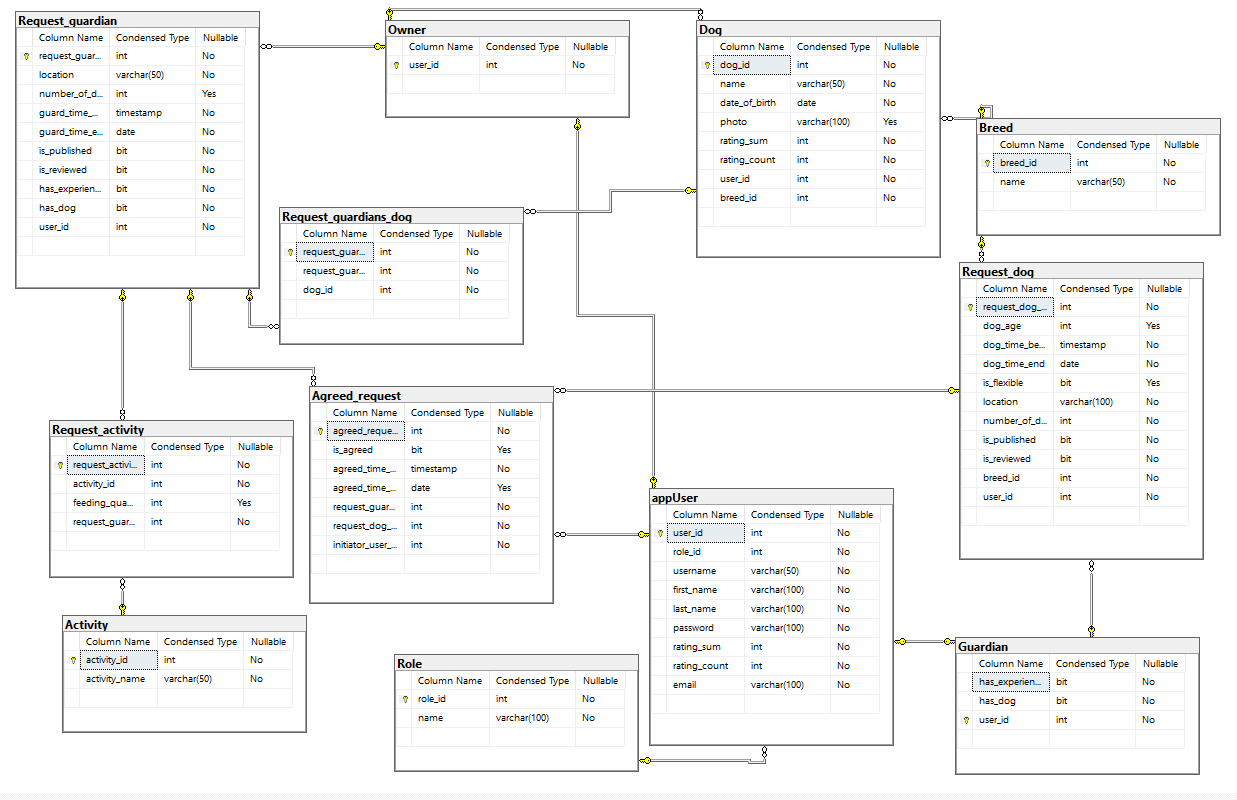
\includegraphics[width=16cm]{slike/dijagramASCP}
				\caption{E-R dijagram baze podataka} 
				\label{fig:E-Rdijagram}
			\end{figure}
			
			\eject
			
			
		\section{Dijagram razreda}
		
			Na slici 4.2 prikazani su razredi koji pripadaju backend dijelu MVC arhitekture.  Zbog lakše organizacije, razredi su podijeljeni logički po pravu pristupa metodama određenih aktora, kako bi se smanjila prenapučenost unutar dijagrama, prikazane su samo ovisnosti između razreda koji pripadaju istom dijelu dijagrama. Iz naziva i tipova atributa u razredima može se zaključiti vrsta ovisnosti među različitim razredima.
			
			\begin{figure}[htb]
				\centering
				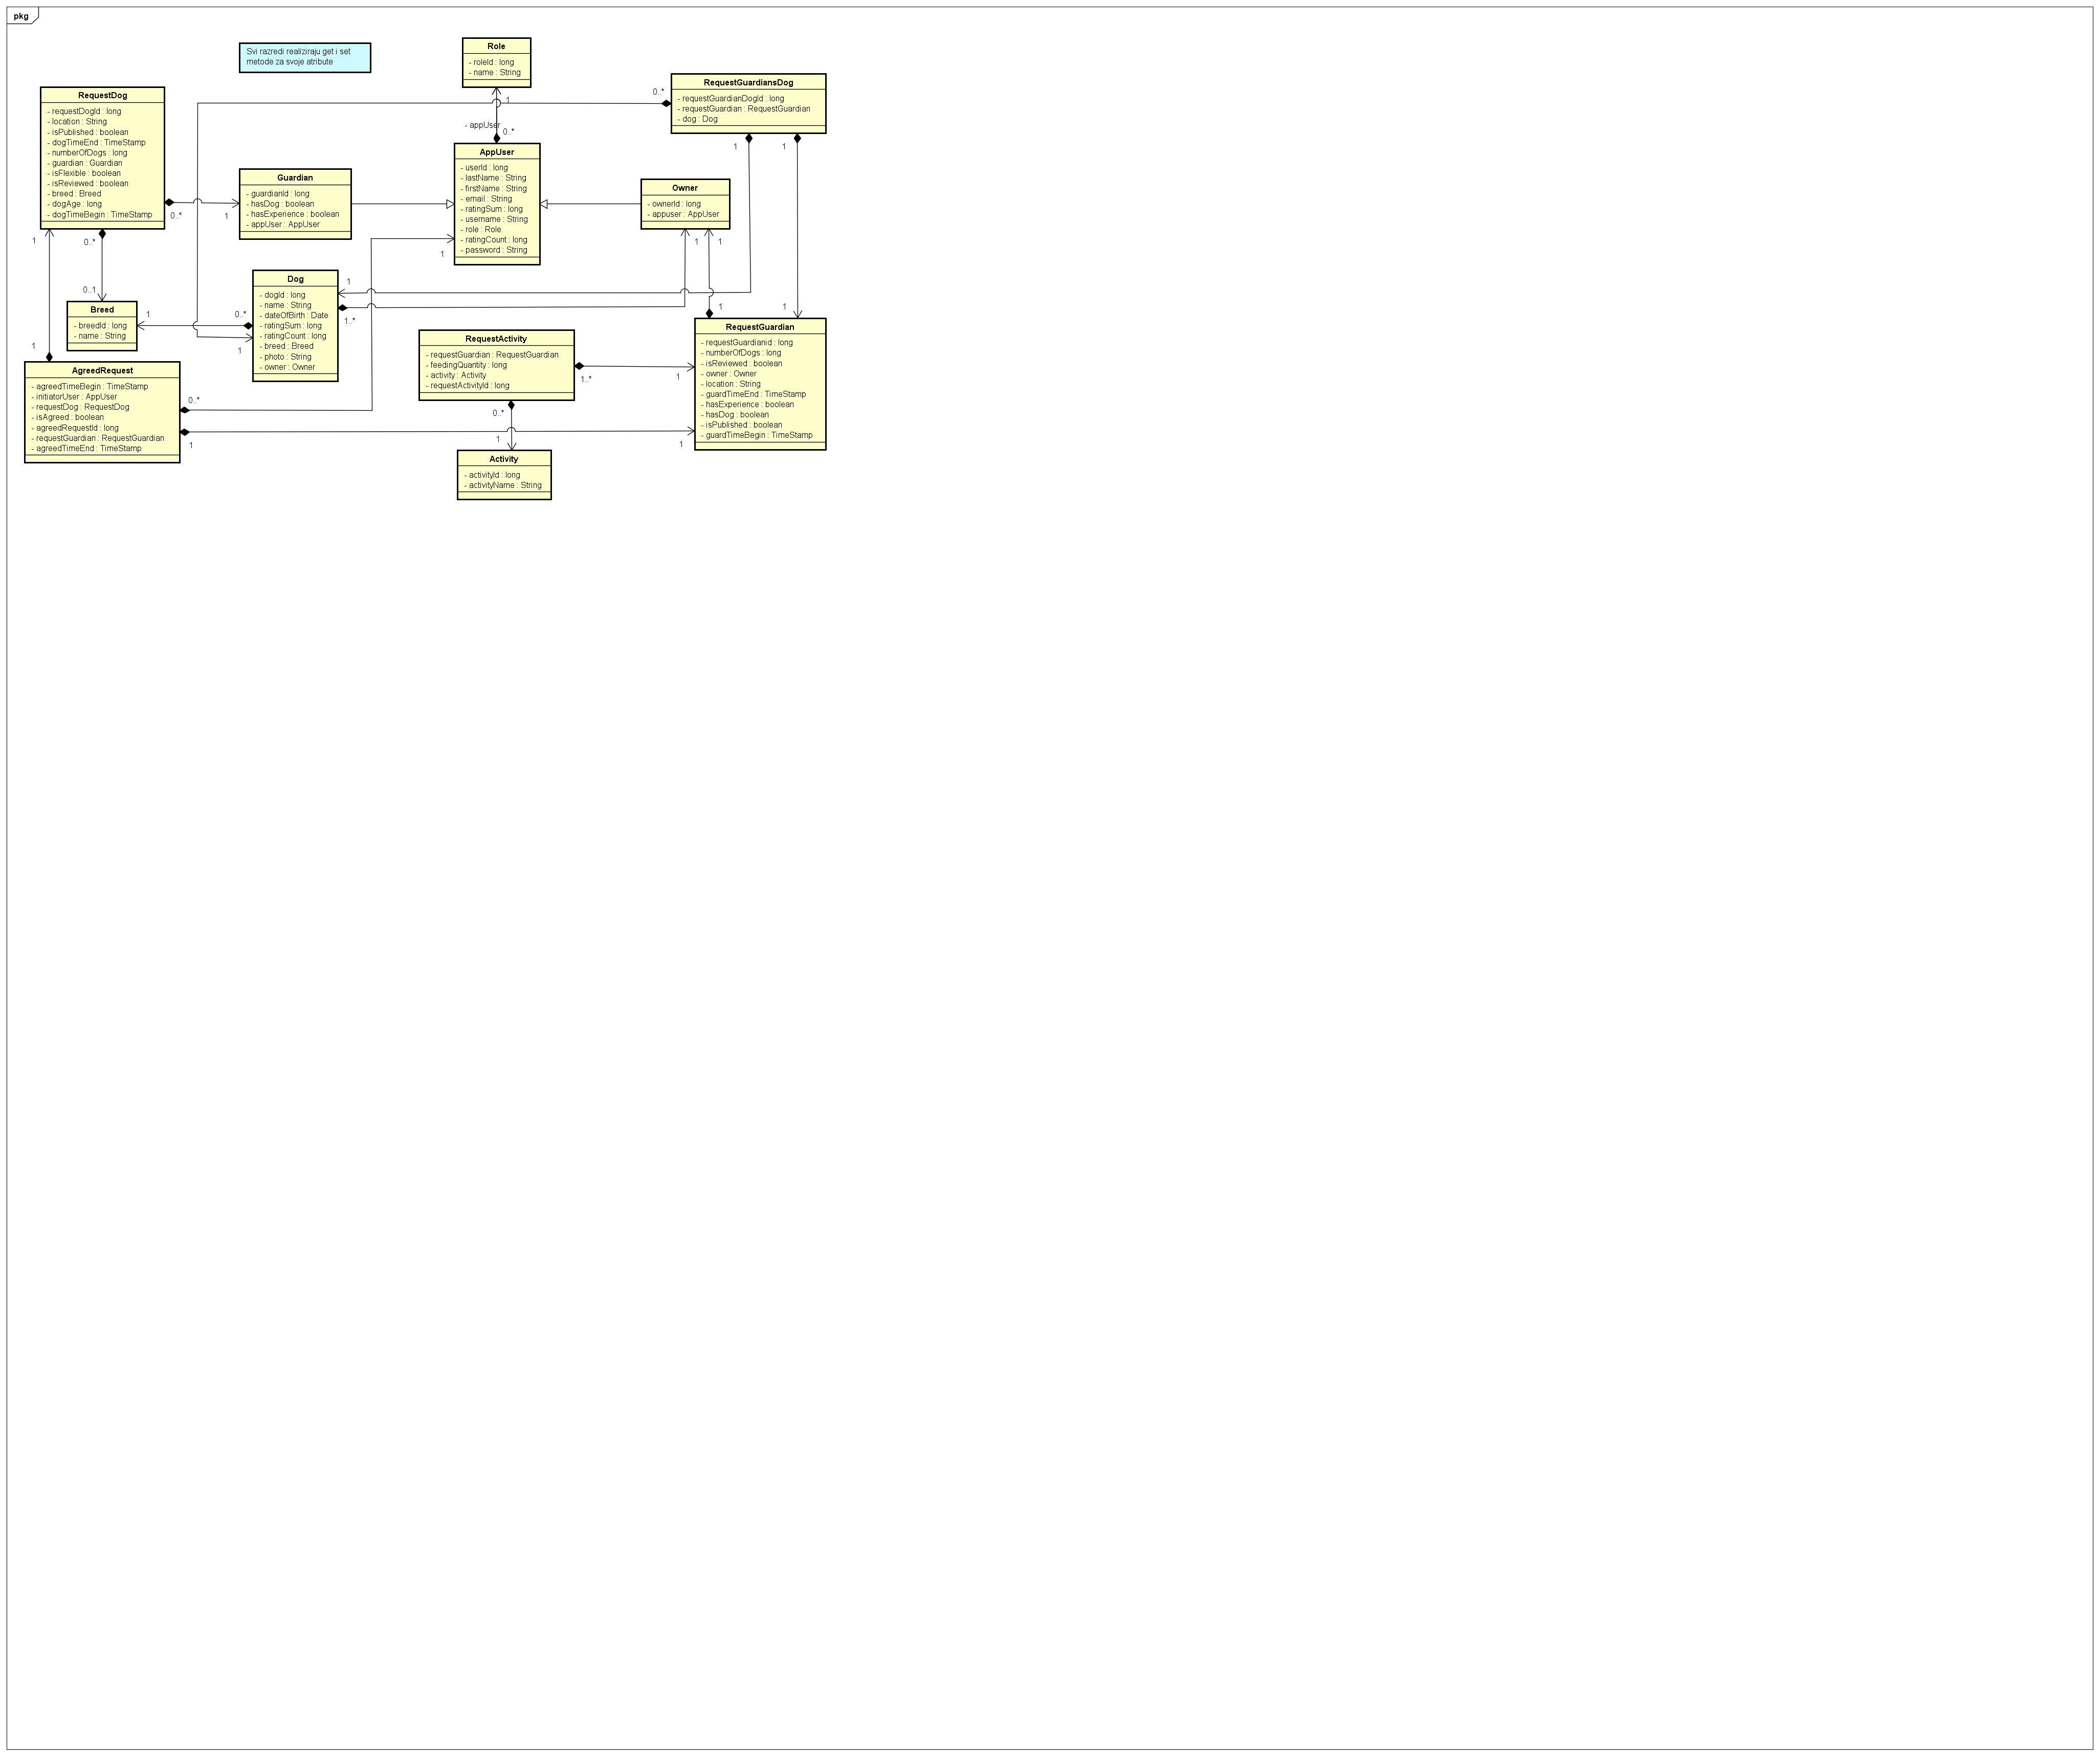
\includegraphics[width=16cm]{slike/Class Diagram}
				\caption{Dijagram razreda - dio Models} 
				\label{fig:Class-Diagram}
			\end{figure}
		
			Model razredi preslikavaju strukturu baze podataka u aplikaciji. Implementirane metode direktno komuniciraju s bazom podataka te vraćaju tražene podatke.\\
			Razred AppUser predstavlja korisnika web aplikacije koji se može registrirati unoseći potrebne informacije. Odabravši pritom rolu (razred Role), on se priključuje web aplikaciji kao vlasnik pasa (razred Owner) i/ili kao čuvar pasa (razred Guardian). Administrator je korisnik aplikacije koji ima sve mogućnosti App Usera. Vlasnik pasa može dodati vlastitog pasa u sustav (razred Dog). Vlasnik i čuvar mogu tražiti čuvara za svog pasa (razred RequestGuardian) odnosno psa za čuvanje (razred RequestDog). Vlasnik može još pregledati ima li čuvar pasa (razred RequestGuardiansDog) i tražiti koju aktivnost će čuvar raditi sa psom (razredi Activity i RequestActivity). Dogovor vlasnika i čuvara predstavlja razred AgreedRequest.
			
			\eject
			
			\textbf{\textit{dio 2. revizije}}\\			
			
			\textit{Prilikom druge predaje projekta dijagram razreda i opisi moraju odgovarati stvarnom stanju implementacije}
			
			
			
			\eject
		
		\section{Dijagram stanja}
			
			
			\textbf{\textit{dio 2. revizije}}\\
			
			\textit{Potrebno je priložiti dijagram stanja i opisati ga. Dovoljan je jedan dijagram stanja koji prikazuje \textbf{značajan dio funkcionalnosti} sustava. Na primjer, stanja korisničkog sučelja i tijek korištenja neke ključne funkcionalnosti jesu značajan dio sustava, a registracija i prijava nisu. }
			
			
			\eject 
		
		\section{Dijagram aktivnosti}
			
			\textbf{\textit{dio 2. revizije}}\\
			
			 \textit{Potrebno je priložiti dijagram aktivnosti s pripadajućim opisom. Dijagram aktivnosti treba prikazivati značajan dio sustava.}
			
			\eject
		\section{Dijagram komponenti}
		
			\textbf{\textit{dio 2. revizije}}\\
		
			 \textit{Potrebno je priložiti dijagram komponenti s pripadajućim opisom. Dijagram komponenti treba prikazivati strukturu cijele aplikacije.}
	\chapter{Implementacija i korisničko sučelje}
		
		
		\section{Korištene tehnologije i alati}
			
			%\textbf{\textit{dio 2. revizije}}
			
			 %\textit{Detaljno navesti sve tehnologije i alate koji su primijenjeni pri izradi dokumentacije i aplikacije. Ukratko ih opisati, te navesti njihovo značenje i mjesto primjene. Za svaki navedeni alat i tehnologiju je potrebno \textbf{navesti internet poveznicu} gdje se mogu preuzeti ili više saznati o njima}.
			
			Frontend aplikacije pisan je u programskom jeziku \textbf{\href{https://www.javascript.com/}{JavaScript}} uz pomoć biblioteke \textbf{\href{https://reactjs.org/}{React}}. React je  open-source JavaScript biblioteka za izgradnju komponenti korisničkog sučelja te je odgovorna samo za prezentacijski sloj aplikacije. Glavni cilj Reacta je razvoj korisničkog sučelja koje poboljšava brzinu aplikacija, pa stoga koristi virtualni DOM (Document Object Model) koji je brži od običnog DOM-a. Aplikacije pisane u Reactu su jednostranične što također pridonosi brzini. Korištenjem komponenti u Reactu, poboljšava se čitljivost i olakšava se održavanje većih aplikacija. React je razvijen od strane Facebooka te korišten i u njihovim aplikacijama poput Instagrama i WhatsAppa.\\
			Kao razvojno okruženje za frontend aplikacije korišten je \textbf{\href{https://code.visualstudio.com/}{Visual Studio Code}}. Visual Studio Code je lagan, ali moćan uređivač izvornog koda razvijen od strane tvrtke Microsoft. Neke od glavnih značajki alata su podrška za ispravljanje pogrešaka, isticanje sintakse, inteligentno dovršavanje koda i mnoge druge. Dolazi s ugrađenom podrškom za JavaScript, TypeScript i Node.js, a ima i bogat ekosustav proširenja za druge jezike i okruženja kao što su C++, C\#, Java, Python, PHP, Go, .NET itd.\\
			Backend aplikacije pisan je u programskom jeziku \textbf{\href{https://www.java.com/en/}{Java}} uz pomoć radnog okvira \textbf{\href{https://spring.io/projects/spring-boot}{Spring Boot}}. Spring Boot je vrlo popularan radni okvir za izgradnju samostojećih aplikacija koje koriste Spring. Spring Boot je specijalizacija radnog okvira Spring razvijen s ciljem jednostavnijeg i bržeg oblikovanja web aplikacija, pa stoga u svojoj automatskoj konfiguraciji olakšava posao programeru jer neke stvari, kao npr. servleti, rad s JSON datotekama, rad s bazama podataka itd., koje su karakteristične za većinu web aplikacja ima automatski podešeno. \\
			Kao razvojno okruženje za backend aplikacije korišten je \textbf{\href{https://www.jetbrains.com/idea/}{IntelliJ IDEA}}. IntelliJ IDEA je integrirano razvojno okruženje (IDE) razvijeno od strane tvrtke JetBrains. Samo razvojno okruženje pisano je u Javi s ciljem poboljšanog razvoja softvera u jezicima Java, Kotlin, Groovy i sl. Ovaj IDE pruža značajke kao što su dovršavanje koda analizom konteksta, navigacija u kodu pri čemu je moguće izravno skakanje na klasu ili deklaraciju u kodu, refaktoriranje koda, otklanjanje pogrešaka i brojne druge. IntelliJ IDEA također podržava dodatke pomoću kojih se može ostvariti dodatna funkcionalnost. Dodaci se mogu preuzeti i instalirati putem njihovog web repozitorija dodataka ili putem IDE-ove ugrađene opcije instaliranja dodataka.\\
			Baza podataka je izvedena u \textbf{\href{https://www.postgresql.org/}{PostgreSQL-u}}. PostgreSQL je open-source sustav za upravljanje relacijskim bazama podataka (RDBMS) kojim se proširuje funkcionalnost SQL-a. PostgreSQL nudi transakcije sa okidačima, stranim ključevima, pohranjenim procedurama, automatski ažuriranim prikazima i sl. Transakcije također imaju svojstva atomarnosti, konzistentnosti, izolacije i izdržljivosti (ACID). PostgreSQL dizajniran je da izdrži različita radna opterećenja, od pojedinačnih računa-la, pa sve do skladišta podataka ili web usluga s mnogo istodobnih korisnika. \\
			Kao okruženje za upravljanje bazom podataka korišten je \textbf{\href{https://www.pgadmin.org/}{pgAdmin}}. pgAdmin je open-source grafički alat za administrativno upravljanje PostgreSQL bazama podataka.\\
			Sama dokumentacija je pisana u jeziku \textbf{\href{https://www.latex-project.org/}{LaTex}}. LaTeX je jezik za pisanje strukturiranih tekstova profesionalne kvalitete. Za razliku od nekih programa za obradu teksta s grafičkim sučeljem poput Microsoft Worda, dokumenti se u LaTeXu pišu kao običan tekst s dodanom semantičkom strukturom te se time postiže usredotočenost na sadržaj, ujednačenost izgleda te brži i stabilniji rad.\\
			Kao okruženje za pisanje dokumentaciju korišten je \textbf{\href{https://www.texstudio.org/}{TeXstudio}}. TeXstudio je open-source integrirano okruženje za izradu LaTeX dokumenata. Posjeduje brojne znač-ajke kao što su pogled na strukturu dokumenta, napredno isticanje sintakse, interaktivna provjera pravopisa, gramatike i referenci, jasan pogled na upozorenja i greške u dokumentu itd.\\
			Za izradu UML dijagrama unutar dokumentacije korišteno je okruženje \textbf{\href{https://astah.net/products/astah-uml/}{Astah UML}}. Astah UML je grafički alat koji je jednostavan za rukovanje te se koristi za izradu potrebnih UML dijagrama. Ima podršku za stvaranje brojnih dijagrama, a samo neki od njih su dijagrami obrazaca uporabe, sekvencijski dijagrami, dijagrami razreda, dijagrami stanja, dijagrami aktivnosti, dijagrami komponenti te dijagrami razmještaja za čiju je izradu alat i korišten.\\
			Za izradu dijagrama baze podataka unutar dokumentacije korišten je online alat \textbf{\href{https://drawsql.app/}{DrawSQL}}.\\
			Kao sustav za upravljanje verzijama projekta korišten je \textbf{\href{https://git-scm.com/}{Git}}. Git je open-source distribuirani sustav za upravljanje različitim verzijama datoteka. Obično se koristi za koordinaciju rada među programerima koji zajednički razvijaju neki softver. Cilj Gita je brzina, integritet podataka i podrška za distribuirane i nelinearne tijekove rada. Svaki Git direktorij na bilo kojem računalu je spremište s potpunom poviješću i punim mogućnostima praćenja verzija.\\
			Udaljeni repozitorij projekta dostupan je na web platformi u oblaku \textbf{\href{https://gitlab.com/}{GitLab}}. GitLab je open-source end-to-end platforma u oblaku za razvoj softvera s ugrađenom kontrolom verzija, praćenjem problema, pregledom koda, CI/CD-om i više.\\
			Za deploy aplikacije korišten je \textbf{\href{https://render.com/}{Render}}. Render je objedinjeni sustav u oblaku koji služi za izgradnju i pokretanje web aplikacija i aplikacija općenito. Pruža pogodnosti poput besplatnih TLS (Transport Layer Security) certifikata, globalnog CDN-a (Content Delivery Network), DDoS (Distributed Denial of Service) zaštite, privatnih mreža i automatske implementacije iz Gita.\\
			Za komunikaciju u timu korišten je \textbf{\href{https://discord.com/}{Discord}}. Discord je društvena platforma na kojoj korisnici imaju mogućnost komuniciranja glasovnim pozivima, videopozivima, tekstualnim porukama, medijima i datotekama u prvatnim razgovorima ili kao dio zajednica koje se nazivaju serveri. Server je skup soba za razgovor i glasovnih kanala te mu je moguće pristupiti putem pozivnice.\\
			
			
			\eject 
		
	
		\section{Ispitivanje programskog rješenja}
			
			\textbf{\textit{dio 2. revizije}}\\
			
			 \textit{U ovom poglavlju je potrebno opisati provedbu ispitivanja implementiranih funkcionalnosti na razini komponenti i na razini cijelog sustava s prikazom odabranih ispitnih slučajeva. Studenti trebaju ispitati temeljnu funkcionalnost i rubne uvjete.}
	
			
			\subsection{Ispitivanje komponenti}
			\textit{Potrebno je provesti ispitivanje jedinica (engl. unit testing) nad razredima koji implementiraju temeljne funkcionalnosti. Razraditi \textbf{minimalno 6 ispitnih slučajeva} u kojima će se ispitati redovni slučajevi, rubni uvjeti te izazivanje pogreške (engl. exception throwing). Poželjno je stvoriti i ispitni slučaj koji koristi funkcionalnosti koje nisu implementirane. Potrebno je priložiti izvorni kôd svih ispitnih slučajeva te prikaz rezultata izvođenja ispita u razvojnom okruženju (prolaz/pad ispita). }
			
			
			
			\subsection{Ispitivanje sustava}
			
			 \textit{Potrebno je provesti i opisati ispitivanje sustava koristeći radni okvir Selenium\footnote{\url{https://www.seleniumhq.org/}}. Razraditi \textbf{minimalno 4 ispitna slučaja} u kojima će se ispitati redovni slučajevi, rubni uvjeti te poziv funkcionalnosti koja nije implementirana/izaziva pogrešku kako bi se vidjelo na koji način sustav reagira kada nešto nije u potpunosti ostvareno. Ispitni slučaj se treba sastojati od ulaza (npr. korisničko ime i lozinka), očekivanog izlaza ili rezultata, koraka ispitivanja i dobivenog izlaza ili rezultata.\\ }
			 
			 \textit{Izradu ispitnih slučajeva pomoću radnog okvira Selenium moguće je provesti pomoću jednog od sljedeća dva alata:}
			 \begin{itemize}
			 	\item \textit{dodatak za preglednik \textbf{Selenium IDE} - snimanje korisnikovih akcija radi automatskog ponavljanja ispita	}
			 	\item \textit{\textbf{Selenium WebDriver} - podrška za pisanje ispita u jezicima Java, C\#, PHP koristeći posebno programsko sučelje.}
			 \end{itemize}
		 	\textit{Detalji o korištenju alata Selenium bit će prikazani na posebnom predavanju tijekom semestra.}
			
			\eject 
		
		
		\section{Dijagram razmještaja}
			
			%\textbf{\textit{dio 2. revizije}}
			
			 %\textit{Potrebno je umetnuti \textbf{specifikacijski} dijagram razmještaja i opisati ga. Moguće je umjesto specifikacijskog dijagrama razmještaja umetnuti dijagram razmještaja instanci, pod uvjetom da taj dijagram bolje opisuje neki važniji dio sustava.}
			 
			 Dijagram razmještaja identificira fizičke i virtualne čvorove koji su prisutni u topologiji sustava te opisuje programsku potporu u implementaciji sustava. Sam sustav baziran je na odnosu klijent-poslužitelj + HTTP protokol za komunikaciju između njih. Cijela poslužiteljska strana ostvarena je pomoću servisa Render.
			 
			 \begin{figure}[H]
			 	\centering
			 	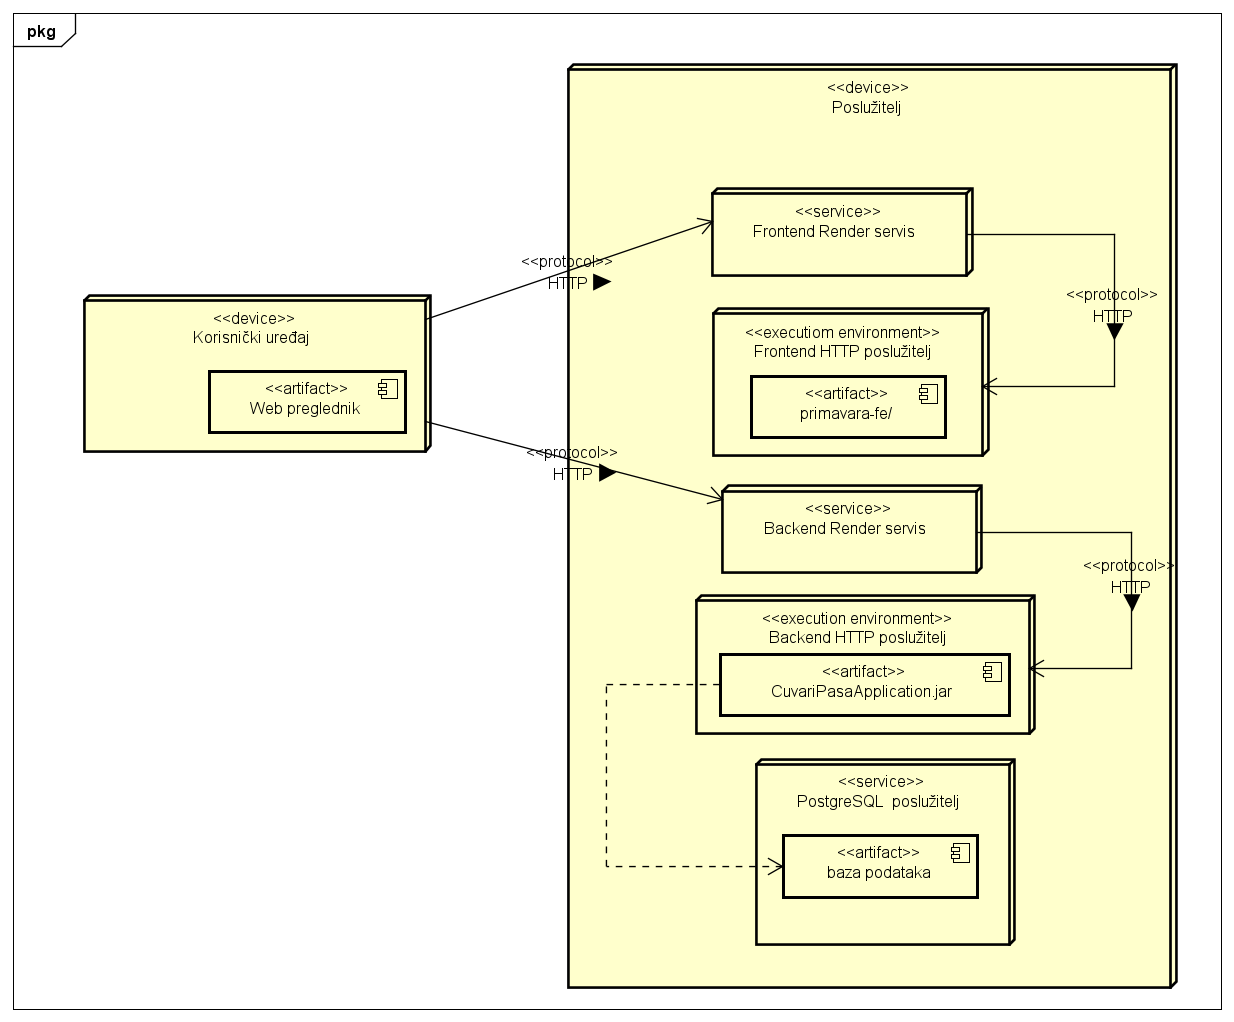
\includegraphics[width=15cm]{slike/dijagramRazmjestaja}
			 	\caption{Dijagram razmještaja}
			 	\label{fig:Activity-Diagram}
			 \end{figure}
			
			\eject 
		
		\section{Upute za puštanje u pogon}
		
			\textbf{\textit{dio 2. revizije}}\\
		
			 \textit{U ovom poglavlju potrebno je dati upute za puštanje u pogon (engl. deployment) ostvarene aplikacije. Na primjer, za web aplikacije, opisati postupak kojim se od izvornog kôda dolazi do potpuno postavljene baze podataka i poslužitelja koji odgovara na upite korisnika. Za mobilnu aplikaciju, postupak kojim se aplikacija izgradi, te postavi na neku od trgovina. Za stolnu (engl. desktop) aplikaciju, postupak kojim se aplikacija instalira na računalo. Ukoliko mobilne i stolne aplikacije komuniciraju s poslužiteljem i/ili bazom podataka, opisati i postupak njihovog postavljanja. Pri izradi uputa preporučuje se \textbf{naglasiti korake instalacije uporabom natuknica} te koristiti što je više moguće \textbf{slike ekrana} (engl. screenshots) kako bi upute bile jasne i jednostavne za slijediti.}
			
			
			 \textit{Dovršenu aplikaciju potrebno je pokrenuti na javno dostupnom poslužitelju. Studentima se preporuča korištenje neke od sljedećih besplatnih usluga: \href{https://aws.amazon.com/}{Amazon AWS}, \href{https://azure.microsoft.com/en-us/}{Microsoft Azure} ili \href{https://www.heroku.com/}{Heroku}. Mobilne aplikacije trebaju biti objavljene na F-Droid, Google Play ili Amazon App trgovini.}
			
			
			\eject 
	\chapter{Zaključak i budući rad}
		
		%\textbf{\textit{dio 2. revizije}}\\
		
		 %\textit{U ovom poglavlju potrebno je napisati osvrt na vrijeme izrade projektnog zadatka, koji su tehnički izazovi prepoznati, jesu li riješeni ili kako bi mogli biti riješeni, koja su znanja stečena pri izradi projekta, koja bi znanja bila posebno potrebna za brže i kvalitetnije ostvarenje projekta i koje bi bile perspektive za nastavak rada u projektnoj grupi.}
		
		 %\textit{Potrebno je točno popisati funkcionalnosti koje nisu implementirane u ostvarenoj aplikaciji.}
		
		Zadatak našeg tima bio je razvoj web aplikacije za traženje i pružanje usluga čuvanja pasa te međusobnu interakciju korisnika prije početka i nakon završetka čuvanja. U protekla 3 mjeseca, svakog tjedna smo radili na razvoju projekta te time ostvarili glavninu funkcionalnosti koje su bile na početku planirane, a usput smo stekli brojna nova i korisna iskustva. Sami razvoj projekta bio je podijeljen u dvije faze, od kojih je prva bila više organizacijske naravi, dok je druga bila potpuno fokusirana na razvoj i implementaciju samog rješenja.\\
		Na početku prve faze slijedilo je okupljanje tima te međusobno upoznavanje, a zatim smo dobili uvid u projektni zadatak koji je bilo potrebno provesti u djelo. Potom smo uz nekoliko timskih sastanaka putem platforme Discord razjasnili i prokomentirali samu suštinu problema te smo na vrlo visokoj razini apstrakcije izradili izgled nekih stranica aplikacije kako bi svi članovi tima dobili dojam o tome kako bi naša aplikacija otprilike funkcionirala. Nakon toga smo krenuli na podjelu poslova i organizaciju u pojedinim podtimovima. Tim je bio podijeljen na podtimove zadužene za razvoj frontenda i backenda te podtim koji se bavi povezivanjem odgovarajućih frontend i backend komponenti. Detaljnije funkcionalnosti koje aplikacija mora obavljati razradili smo kroz funkcionalne zahtjeve i obrasce uporabe te pripadajuće dijagrame koji su nam uvelike pomogli i olakšali daljnji razvoj aplikacije. Pošto većina članova tima prethodno nije bila upoznata s pojedinim tehnologijama koje smo planirali koristiti za razvoj, kroz niz tehničkih radionica i samostalno istraživanje polako smo se upoznavali sa potrebnim alatima i načinom na koji ih trebamo koristiti. Na kraju prve faze ostvarili smo generičke funkcionalnosti kao što su prijava i registracija u sustav te pripadajući dizajn i izgled tih stranica.\\
		Dolazimo do druge faze u kojoj stvari postaju malo zahtjevnije zbog nekih faktora kao što su količina funkcionalnosti koje je još bilo potrebno ostvariti te vremenski period koji nam je bio na raspolaganju za njihovo ostvarenje. U narednim tjednima rad na aplikaciji i samoj dokumentaciji bio je mnogo intenzivniji. Preostalo je dokumentirati podosta poglavlja te izraditi dijagrame koji odgovaraju radu naše aplikacije. Uz to, kao i uvijek, naišli smo i na neke probleme u razvoju koji su iziskivali puno vremena da se nađe odgovarajuće rješenje. Usprkos tome, na vrijeme smo bili gotovi s ostvarenjem planiranih funkcionalnosti naše aplikacije i nakon toga preostalo je dovršiti izgled same aplikacije te neke sitne preinake kako bi sve bilo ispravno i u funkciji.\\
		Na samom kraju, zadovoljni smo onime što smo postigli i napravili. Svakako najbitnije od svega je iskustvo koje smo stekli tokom rada na ovom projektu. Timski rad te međusobna komunikacija i organizacija je ono što nam je pomoglo da dođemo do završnog proizvoda. Izrada samog projekta vjerojatno bi bila dosta brža i bezbolnija da smo prethodno bili upoznati s korištenim tehnologijama. No, zato smo kroz ovaj projekt dobili potrebna znanja i vjetar u leđa za buduće projekte.\\
		
		
		\eject 
	\chapter*{Popis literature}
		\addcontentsline{toc}{chapter}{Popis literature}
	 	
 	
		
		
		\begin{enumerate}
			
			
			\item  Programsko inženjerstvo, FER ZEMRIS, \url{http://www.fer.hr/predmet/proinz}
			
			\item  I. Sommerville, "Software engineering", 8th ed, Addison Wesley, 2007.
			
			\item  T.C.Lethbridge, R.Langaniere, "Object-Oriented Software Engineering", 2nd ed. McGraw-Hill, 2005.
			
			\item  I. Marsic, Software engineering book``, Department of Electrical and Computer Engineering, Rutgers University, \url{http://www.ece.rutgers.edu/~marsic/books/SE}
			
			\item  The Unified Modeling Language, \url{https://www.uml-diagrams.org/}
			
			\item  Astah Community, \url{http://astah.net/editions/uml-new}
		\end{enumerate}
		
		 
	
	
	\begingroup
	\renewcommand*\listfigurename{Indeks slika i dijagrama}
	%\renewcommand*\listtablename{Indeks tablica}
	%\let\clearpage\relax
	\listoffigures
	%\vspace{10mm}
	%\listoftables
	\endgroup
	\addcontentsline{toc}{chapter}{Indeks slika i dijagrama}


	
	\eject 
		
	\chapter*{Dodatak: Prikaz aktivnosti grupe}
		\addcontentsline{toc}{chapter}{Dodatak: Prikaz aktivnosti grupe}
		
		\section*{Dnevnik sastajanja}
		
		\textbf{\textit{Kontinuirano osvježavanje}}\\
		
		 \textit{U ovom dijelu potrebno je redovito osvježavati dnevnik sastajanja prema predlošku.}
		
		\begin{packed_enum}
			\item  sastanak
			
			\item[] \begin{packed_item}
				\item Datum: u ovom formatu: \today
				\item Prisustvovali: I.Prezime, I.Prezime
				\item Teme sastanka:
				\begin{packed_item}
					\item  opis prve teme
					\item  opis druge teme
				\end{packed_item}
			\end{packed_item}
			
			\item  sastanak
			\item[] \begin{packed_item}
				\item Datum: u ovom formatu: \today
				\item Prisustvovali: I.Prezime, I.Prezime
				\item Teme sastanka:
				\begin{packed_item}
					\item  opis prve teme
					\item  opis druge teme
				\end{packed_item}
			\end{packed_item}
			
			%
			
		\end{packed_enum}
		
		\eject
		\section*{Tablica aktivnosti}
		
			\textbf{\textit{Kontinuirano osvježavanje}}\\
			
			 \textit{Napomena: Doprinose u aktivnostima treba navesti u satima po članovima grupe po aktivnosti.}

			\begin{longtblr}[
					label=none,
				]{
					vlines,hlines,
					width = \textwidth,
					colspec={X[7, l]X[1, c]X[1, c]X[1, c]X[1, c]X[1, c]X[1, c]X[1, c]}, 
					vline{1} = {1}{text=\clap{}},
					hline{1} = {1}{text=\clap{}},
					rowhead = 1,
				} 
				\multicolumn{1}{c|}{} & \multicolumn{1}{c|}{\rotatebox{90}{\textbf{Antonio Lukić}}} & \multicolumn{1}{c|}{\rotatebox{90}{\textbf{Ivan Kapusta }}} &	
				\multicolumn{1}{c|}{\rotatebox{90}{\textbf{Ivan Kuzmić }}} & 
				\multicolumn{1}{c|}{\rotatebox{90}{\textbf{Mario Petek }}} &	
				\multicolumn{1}{c|}{\rotatebox{90}{\textbf{Lovro Malojčić }}} & 
				\multicolumn{1}{c|}{\rotatebox{90}{\textbf{Sven Leko }}} &	
				\multicolumn{1}{c|}{\rotatebox{90}{\textbf{Eugen Preglej }}} \\  
				Upravljanje projektom 		&  &  &  &  &  &  & \\ 
				Opis projektnog zadatka 	&  &  &  &  &  &  & \\ 
				
				Funkcionalni zahtjevi       &  &  &  &  &  &  &  \\ 
				Opis pojedinih obrazaca 	&  &  &  &  &  &  &  \\ 
				Dijagram obrazaca 			&  &  &  &  &  &  &  \\ 
				Sekvencijski dijagrami 		&  &  &  &  &  &  &  \\ 
				Opis ostalih zahtjeva 		&  &  &  &  &  &  &  \\ 

				Arhitektura i dizajn sustava	 &  &  &  &  &  &  &  \\ 
				Baza podataka				&  &  &  &  &  &  &   \\ 
				Dijagram razreda 			&  &  &  &  &  &  &   \\ 
				Dijagram stanja				&  &  &  &  &  &  &  \\ 
				Dijagram aktivnosti 		&  &  &  &  &  &  &  \\ 
				Dijagram komponenti			&  &  &  &  &  &  &  \\ 
				Korištene tehnologije i alati 		&  &  &  &  &  &  &  \\ 
				Ispitivanje programskog rješenja 	&  &  &  &  &  &  &  \\ 
				Dijagram razmještaja			&  &  &  &  &  &  &  \\ 
				Upute za puštanje u pogon 		&  &  &  &  &  &  &  \\  
				Dnevnik sastajanja 			&  &  &  &  &  &  &  \\ 
				Zaključak i budući rad 		&  &  &  &  &  &  &  \\  
				Popis literature 			&  &  &  &  &  &  &  \\  
				&  &  &  &  &  &  &  \\ \hline 
				\textit{Dodatne stavke kako ste podijelili izradu aplikacije} 			&  &  &  &  &  &  &  \\ 
				\textit{npr. izrada početne stranice} 				&  &  &  &  &  &  &  \\  
				\textit{izrada baze podataka} 		 			&  &  &  &  &  &  & \\  
				\textit{spajanje s bazom podataka} 							&  &  &  &  &  &  &  \\ 
				\textit{back end} 							&  &  &  &  &  &  &  \\  
				 							&  &  &  &  &  &  &\\ 
			\end{longtblr}
					
					
		\eject
		\section*{Dijagrami pregleda promjena}
		
		\textbf{\textit{dio 2. revizije}}\\
		
		\textit{Prenijeti dijagram pregleda promjena nad datotekama projekta. Potrebno je na kraju projekta generirane grafove s gitlaba prenijeti u ovo poglavlje dokumentacije. Dijagrami za vlastiti projekt se mogu preuzeti s gitlab.com stranice, u izborniku Repository, pritiskom na stavku Contributors.}
		
	


\end{document} %naredbe i tekst nakon ove naredbe ne ulaze u izgrađen dokument 


